\documentclass[12pt,a4paper]{article}

% --- PAKETE FÜR LAYOUT UND SPRACHE ---
\usepackage[utf8]{inputenc}
\usepackage[ngerman]{babel}
\usepackage[T1]{fontenc}
\usepackage{graphicx}
\usepackage{geometry}
\geometry{margin=2.5cm, top=3cm, bottom=3cm}
\usepackage{listings}
\usepackage{xcolor}
\usepackage{hyperref}
\hypersetup{colorlinks=false, hidelinks}
\usepackage{titlesec}
\usepackage{amsmath}
\usepackage{enumitem}
\usepackage{float}

% --- KOPF- UND FUSSZEILE ---
\usepackage{fancyhdr}
\pagestyle{fancy}
\fancyhf{}

\fancyhead[C]{\textbf{Roboterhand}}
\renewcommand{\headrulewidth}{0.6pt}

\fancyfoot[L]{Projektdokumentation}
\fancyfoot[C]{\textbf{Nisa Nur Sisman \& Branka Tomic}}
\fancyfoot[R]{\thepage}
\renewcommand{\footrulewidth}{0.6pt}

\fancypagestyle{plain}{
    \fancyhf{}
    \renewcommand{\headrulewidth}{0pt}
    \renewcommand{\footrulewidth}{0pt}
}

% --- SCHRIFTART AUF HELVETICA/ARIAL ---
\usepackage{helvet}
\renewcommand{\familydefault}{\sfdefault}

% --- ÜBERSCHRIFTEN-STYLING ---
\titleformat{\section}{\normalfont\large\bfseries}{\thesection}{1em}{}
\titleformat{\subsection}{\normalfont\normalsize\bfseries}{\thesubsection}{1em}{}

% --- CODE-STYLING ---
\definecolor{codegreen}{rgb}{0,0.6,0}
\definecolor{codegray}{rgb}{0.5,0.5,0.5}
\definecolor{codepurple}{rgb}{0.58,0,0.82}
\lstset{
    commentstyle=\color{codegreen},
    keywordstyle=\color{magenta},
    numberstyle=\tiny\color{codegray},
    stringstyle=\color{codepurple},
    basicstyle=\ttfamily\footnotesize,
    breakatwhitespace=false,
    breaklines=true,
    captionpos=b,
    keepspaces=true,
    numbers=left,
    showspaces=false,
    showstringspaces=false,
    showtabs=false,
    tabsize=2
}

% --- BEGINN DES DOKUMENTS ---
\begin{document}

% --- TITELSEITE ---
\begin{titlepage}
    \thispagestyle{empty}
    \centering

    {\huge \textbf{Roboterhand} \par}
    \vspace{0.5cm}

    {\normalsize ESP32-Steuerung mit Flex-Sensoren und KI \par}
    \vspace{1.5cm}

    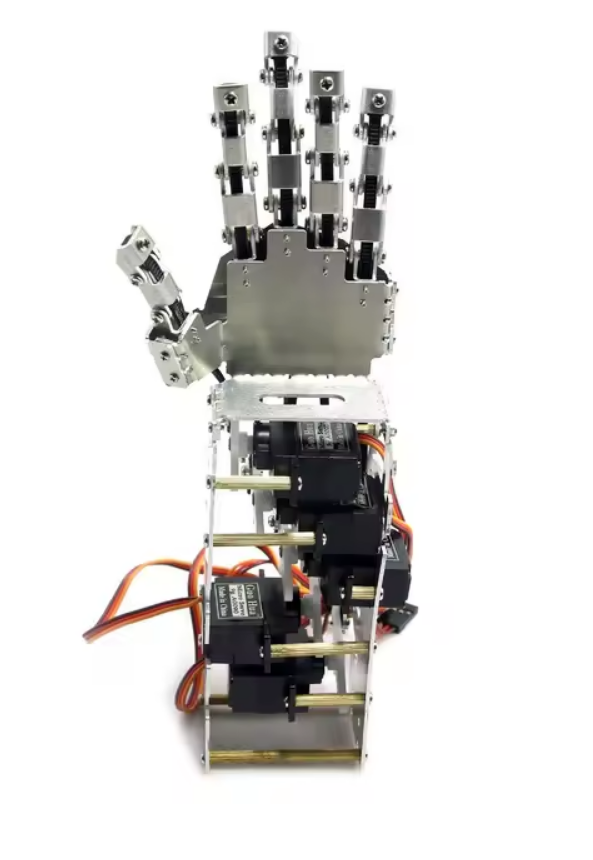
\includegraphics[width=0.6\textwidth]{bilder/handVonVorne.png}
    \vspace{1.5cm}

    {\Large \textbf{Projektdokumentation} \par}
    \vspace{1cm}

    {\large Vorgelegt von:} \\[0.3cm]
    {\textbf{Nisa Nur Sisman}} \\[0.3cm]
    {\textbf{Branka Tomic}} \\
    \vspace{0.6cm}

    {\normalsize \today \par}
\end{titlepage}

% --- INHALTSVERZEICHNIS ---
\tableofcontents
\newpage

% ============================================================
% 1. EINLEITUNG
% ============================================================
\section{Einleitung}

In diesem Projekt wird eine interaktive Roboterhand auf Basis eines ESP32-Mikrocontrollers 
realisiert, die über drei unabhängige Steuerungsmodi bedient werden kann: einen 
Handschuh mit Flex-Sensoren, eine webbasierte Benutzeroberfläche sowie eine 
KI-gestützte Kameraerkennung mit MediaPipe. Das Projekt verbindet Elektronik, 
Embedded-Programmierung und Künstliche Intelligenz zu einem praxisnahen System, 
das menschliche Fingerbewegungen in Echtzeit auf eine mechanische Hand überträgt.

\subsection{Ziel des Projekts}
Das Ziel dieses Projekts ist es, eine funktionsfähige Roboterhand zu entwickeln, 
die Fingerbewegungen eines Menschen präzise nachahmt. Das System soll Sensordaten 
in Echtzeit verarbeiten, die Servomotoren zuverlässig ansteuern und zwischen 
verschiedenen Steuerungsmodi wechseln können. Gleichzeitig soll es praxisnahe 
Erfahrungen in Mikrocontroller-Programmierung, Sensorverarbeitung und 
Human-Machine-Interaction vermitteln.

\subsection{Motivation}
Wir haben dieses Thema gewählt, weil uns die Verbindung zwischen Mensch und 
Maschine fasziniert. Der Auslöser war eine Hochschulmesse an der Technischen 
Hochschule Mannheim, auf der ein ähnliches Projekt ausgestellt war. Die Idee, 
eigene Fingerbewegungen direkt auf eine mechanische Hand zu übertragen, hat uns 
sofort begeistert. Durch die schrittweise Erweiterung um eine Website-Steuerung 
und eine KI-Komponente konnten wir zusätzlich Erfahrungen in Webentwicklung 
und Computer Vision sammeln.

% ============================================================
% 2. ORGANISATION
% ============================================================
\newpage

\section{Organisation}
Zur Planung und Aufgabenverteilung wurde GanttProject eingesetzt. Damit konnten 
die Arbeitsphasen zeitlich strukturiert und die Aufgaben gleichmäßig auf beide 
Projektmitglieder verteilt werden.

\subsection{Zeitplanung}

\begin{table}[h]
\centering
\renewcommand{\arraystretch}{1.3}
\begin{tabular}{|c|l|l|}
\hline
\textbf{Phase} & \textbf{Zeitraum (geplant)} & \textbf{Inhalt} \\
\hline
1 & 20.10.2025 -- 09.11.2025 & Komponentenwahl und Recherche \\
\hline
2 & 10.11.2025 -- 07.12.2025 & Hardware-Aufbau, Verkabelung, \\
  &                           & Handschuh-Konstruktion, D-Sub-Verdrahtung \\
\hline
3 & 08.12.2025 -- 21.12.2025 & Flex-Sensor-Code, Kalibrierung, \\
  &                           & MedianFilter, Diff-Prinzip \\
\hline
4 & 05.01.2026 -- 22.03.2026 & Gesamttests, Fehlersuche, \\
  &                           & Feinabstimmung \\
\hline
5 & 23.03.2026 -- 29.04.2026 & Dokumentation finalisieren, \\
  &                           & Präsentation vorbereiten, Abgabe \\
\hline
+ & 05.01.2026 -- 22.03.2026 & Zusätzliche Erweiterungen\\
\hline
\end{tabular}
\caption{Geplanter Projektzeitplan (20.10.2025 -- 29.04.2026)}
\end{table}

\subsection{Arbeitspakete}
Die anfallenden Aufgaben wurden entsprechend der Stärken beider Projektmitglieder aufgeteilt. Die folgende Übersicht zeigt, wer für welche Bereiche verantwortlich war:

\begin{table}[h]
\centering
\begin{tabular}{|l|l|l|}
\hline
\textbf{Bereich} & \textbf{Aufgabe} & \textbf{Verantwortlich} \\
\hline
Konzeption & Recherche, Komponentenwahl & Gemeinsam \\
Hardware & Verkabelung, Handschuh-Aufbau & Branka \\
Programmierung & ESP32-Code, Modus-Steuerung & Nisa \\
Website & Funktionale Umsetzung & Branka \\
Website & Gestalterische Umsetzung & Branka \\
Sensorik & Flex-Sensor-Code, MedianFilter, Diff-Prinzip & Nisa \\
KI-Modus & MediaPipe-Integration & Nisa \\
KI-Modus & Serielle Datenübertragung & Branka \\
Dokumentation & Ausarbeitung, Präsentation & Gemeinsam \\
\hline
\end{tabular}
\caption{Aufgabenverteilung im Projekt}
\end{table}

\newpage

% ============================================================
% 3. STEUERUNGS-MODI
% ============================================================
\section{Steuerungs-Modi}

In diesem Kapitel werden die drei realisierten Steuerungsmodi im Detail beschrieben. Dabei wird auf den jeweiligen Ablauf aus Benutzerperspektive sowie auf die technische Umsetzung im Hintergrund eingegangen.
Darunter ermöglichen drei Schaltflächen den Wechsel zwischen den verfügbaren Modi 
(Website, Flex-Sensor, Kamera), wobei der aktive Modus als Statustext angezeigt 
wird. Im mittleren Bereich steuern fünf Schieberegler (bzw. zehn im Zwei-Hand-Modus) 
die Servomotoren manuell; diese sind nur im Website-Modus aktiv und werden in den 
anderen Modi deaktiviert. Im unteren Bereich befinden sich Schaltflächen für die 
Posen ,,Peace`` und ,,Faust`` sowie die Möglichkeit, eine eigene Pose zu speichern 
und später wieder abzurufen.

\subsection{Website-Steuerung}
Die Website wird direkt vom ESP32 gehostet und ist über dessen IP-Adresse im lokalen 
Netzwerk erreichbar. Ganz oben befinden sich zwei Schaltflächen zur Auswahl der 
Handanzahl: ,,1 Hand`` und ,,2 Hände``. Durch Drücken von ,,2 Hände`` erweitert 
sich die gesamte Oberfläche -- alle Steuerelemente werden für beide Hände angezeigt.

\vspace{1cm}
\begin{figure}[H]
    \centering
    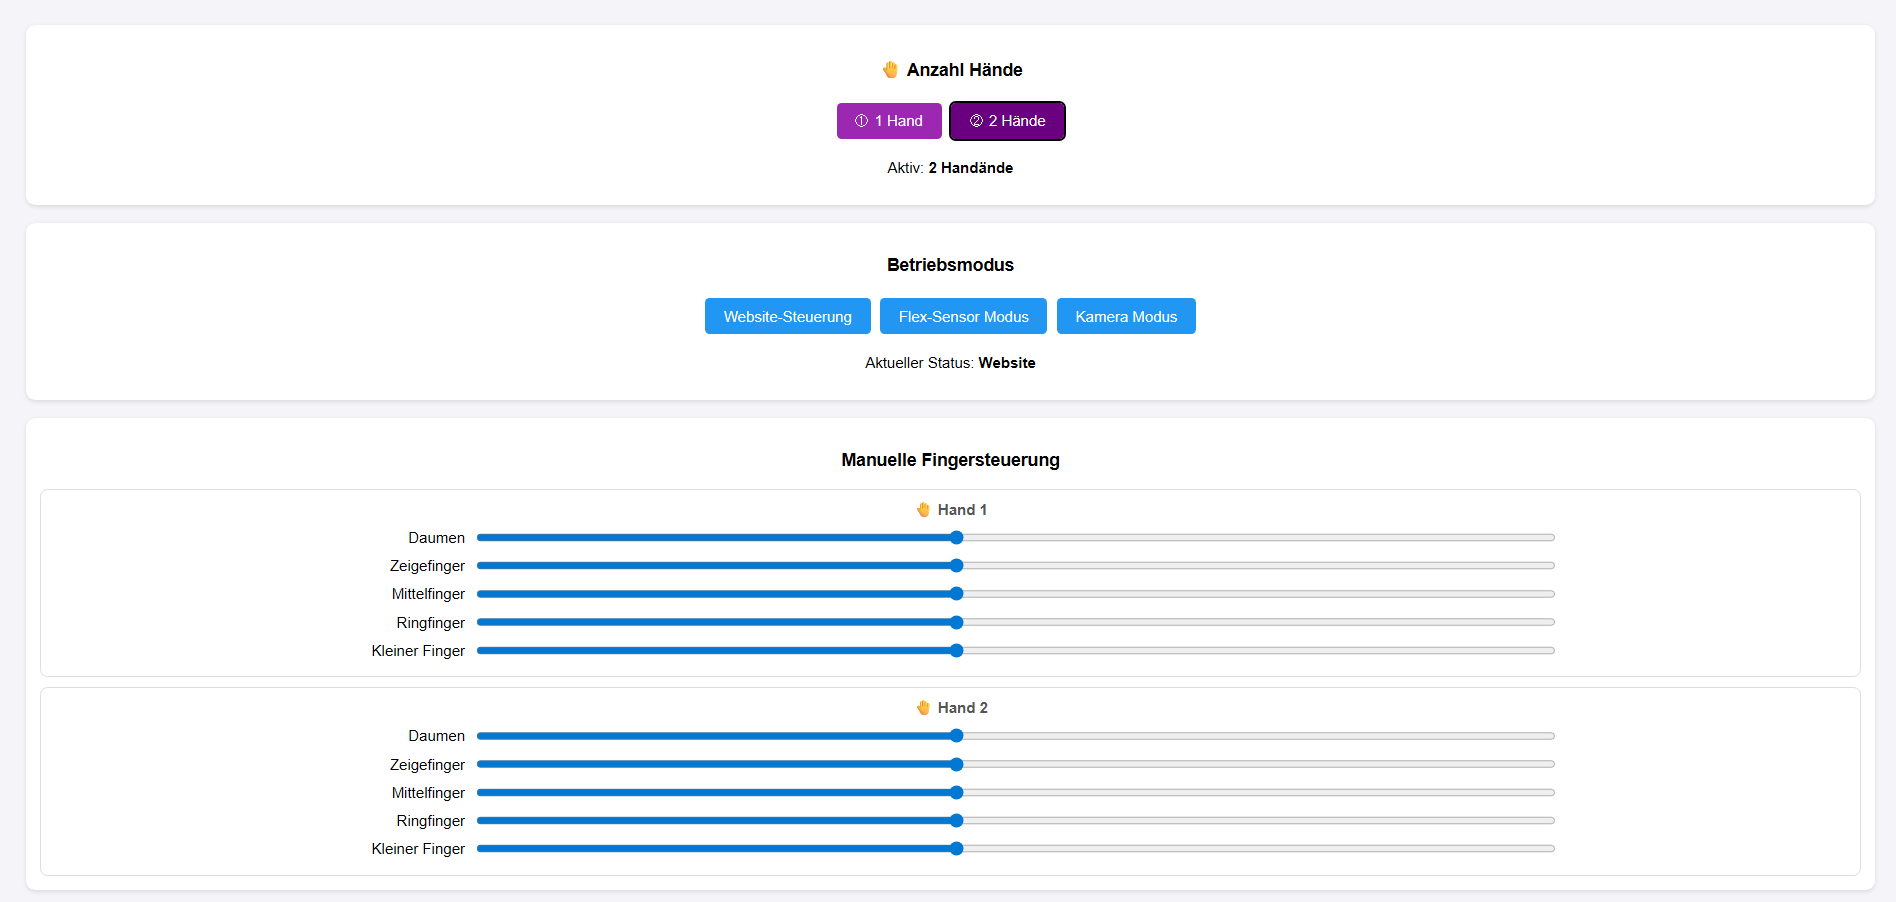
\includegraphics[width=1\textwidth]{bilder/WebsiteScreenshot1.png}
    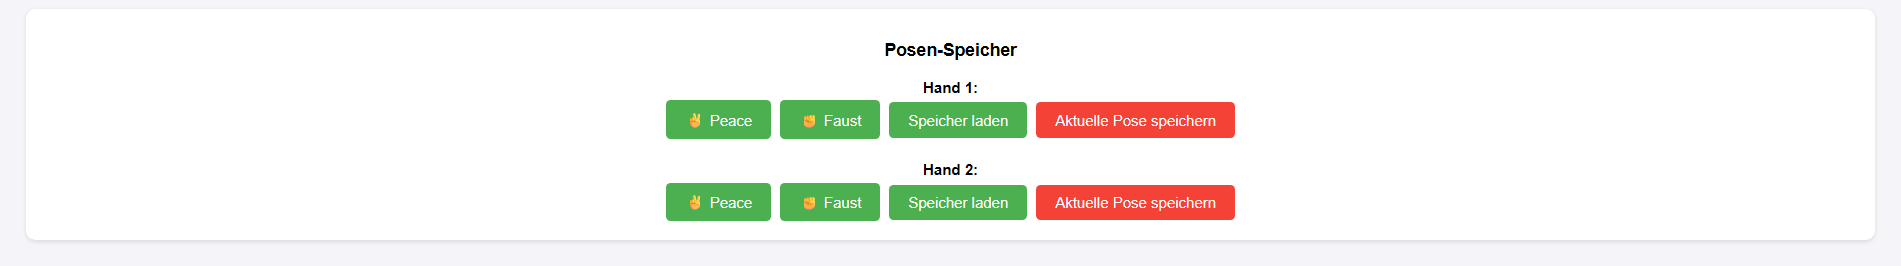
\includegraphics[width=1\textwidth]{bilder/WebsiteScreenshot2.png}
    \caption{Website-Steuerung -- 2-Hände-Modus (PC)}
\end{figure}

\begin{figure}[H]
    \centering
    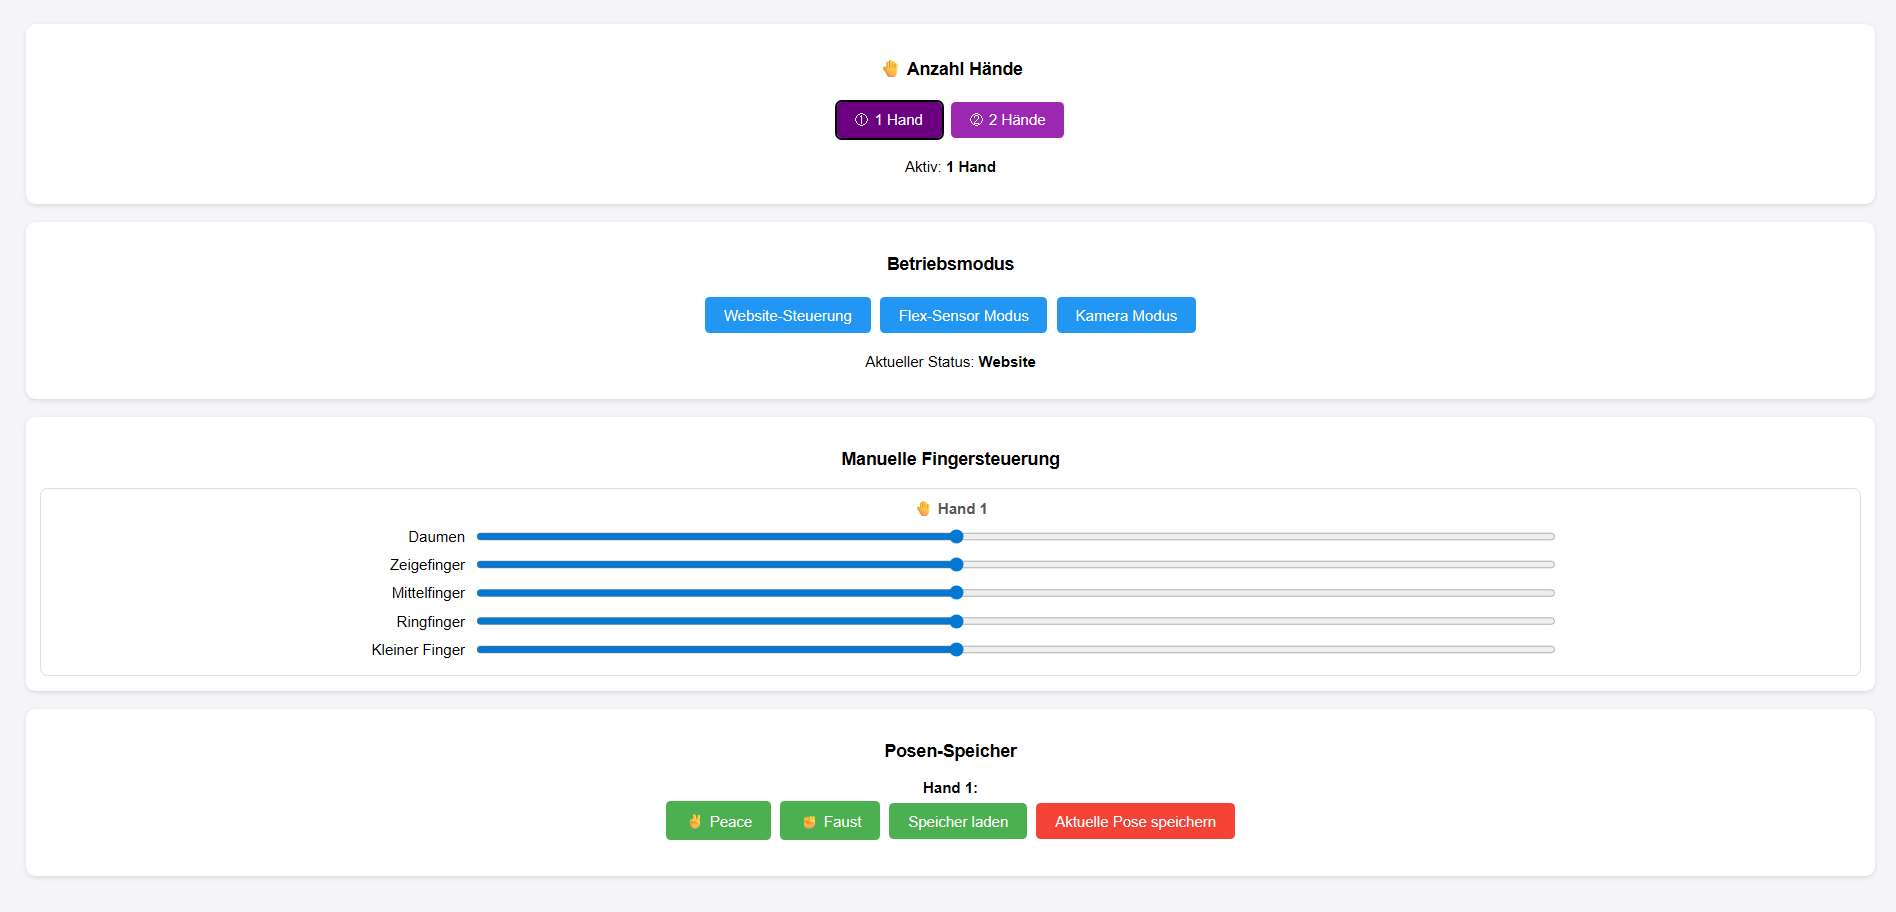
\includegraphics[width=1\textwidth]{bilder/WebsiteScreenshot3.png}
    \caption{Website-Steuerung -- 1-Hand-Modus (PC)}
\end{figure}

\begin{figure}[H]
    \centering
    \begin{minipage}[t]{0.35\textwidth}
        \centering
        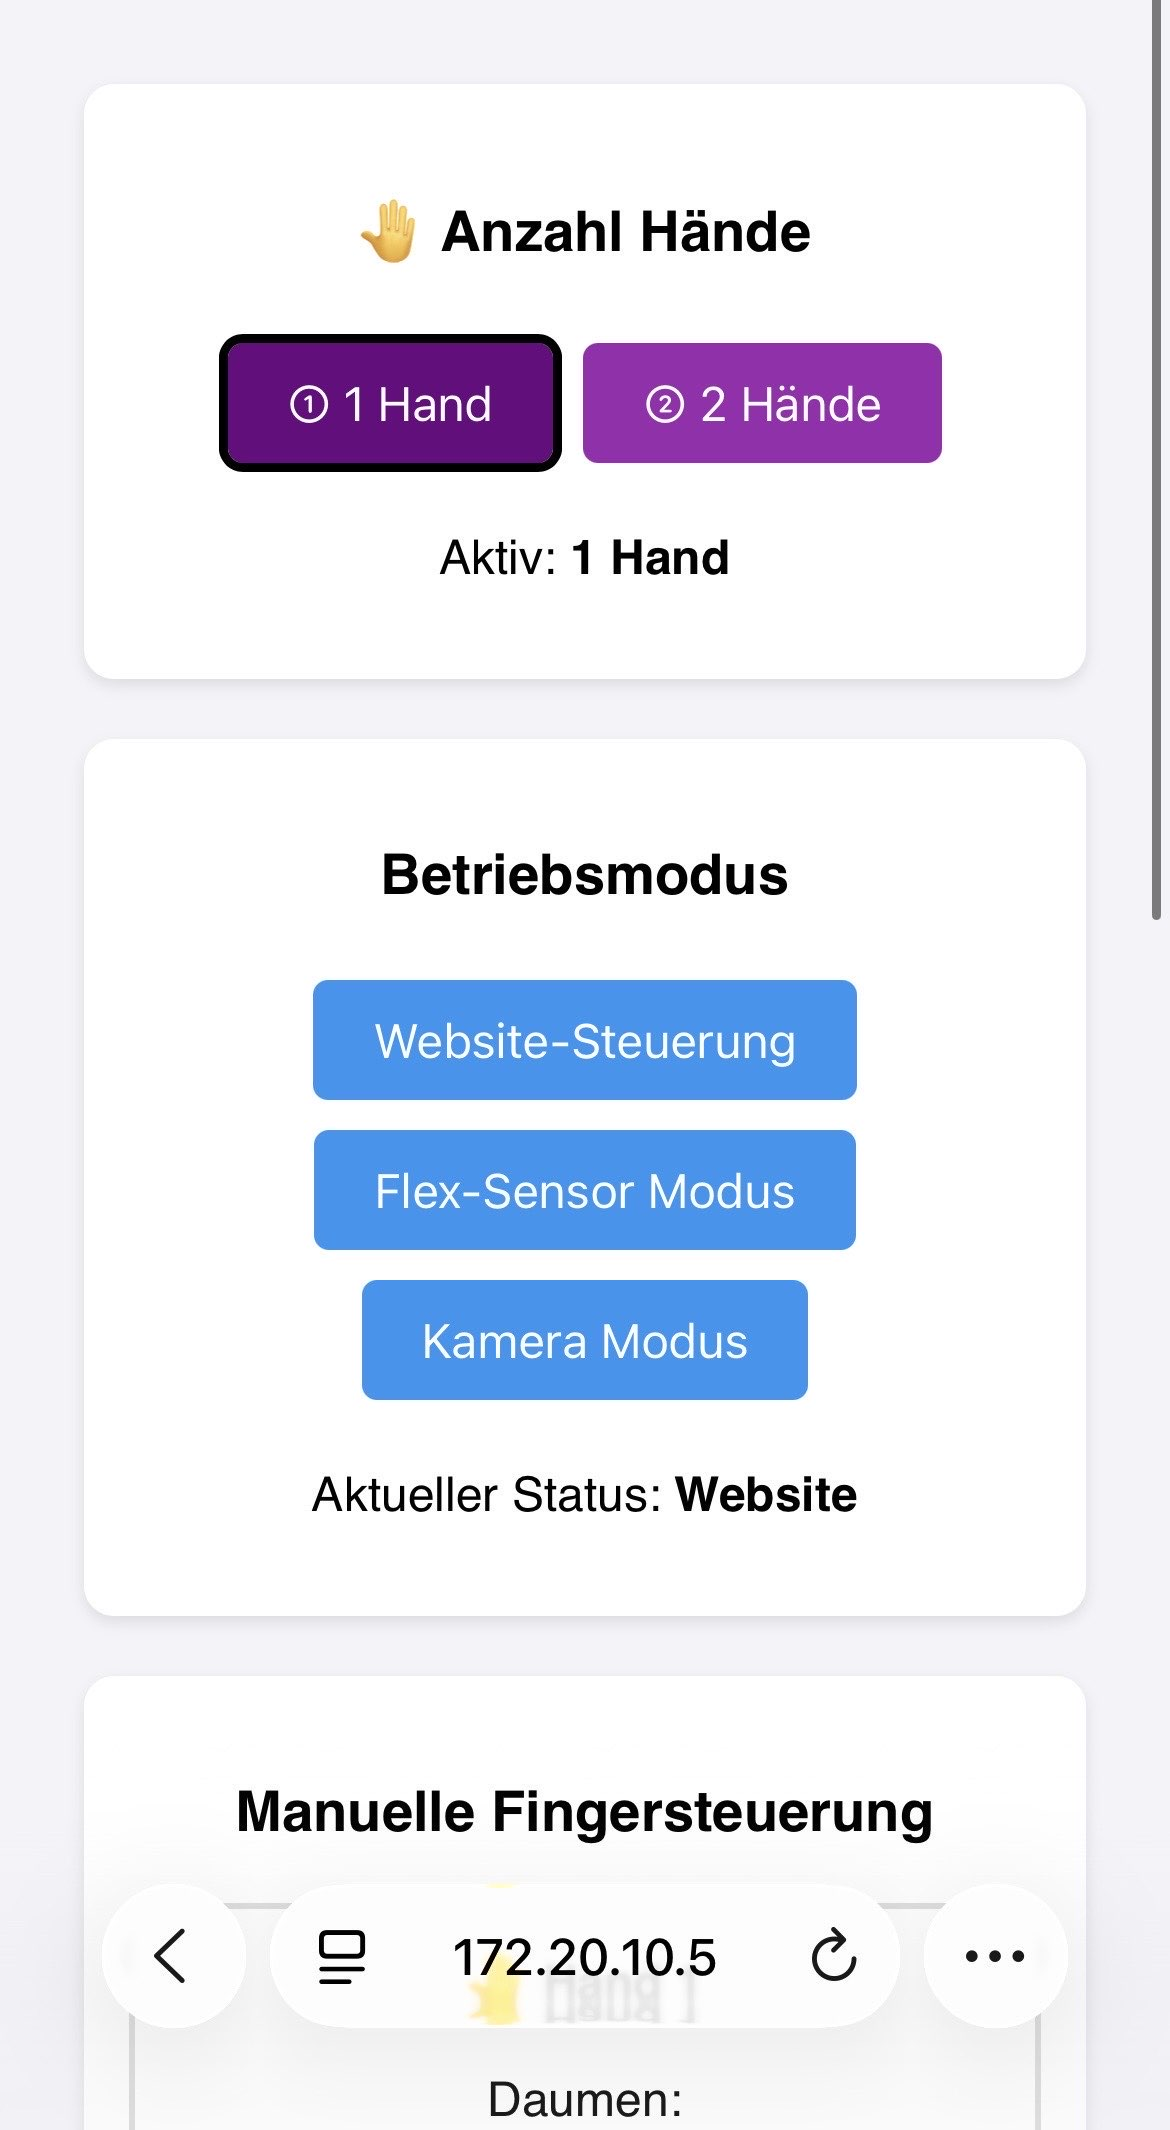
\includegraphics[width=\textwidth]{bilder/webWeb.jpg}
        \caption{Website-Steuerung auf dem Smartphone}
    \end{minipage}
    \hspace{1cm}
    \begin{minipage}[t]{0.3\textwidth}
        \centering
        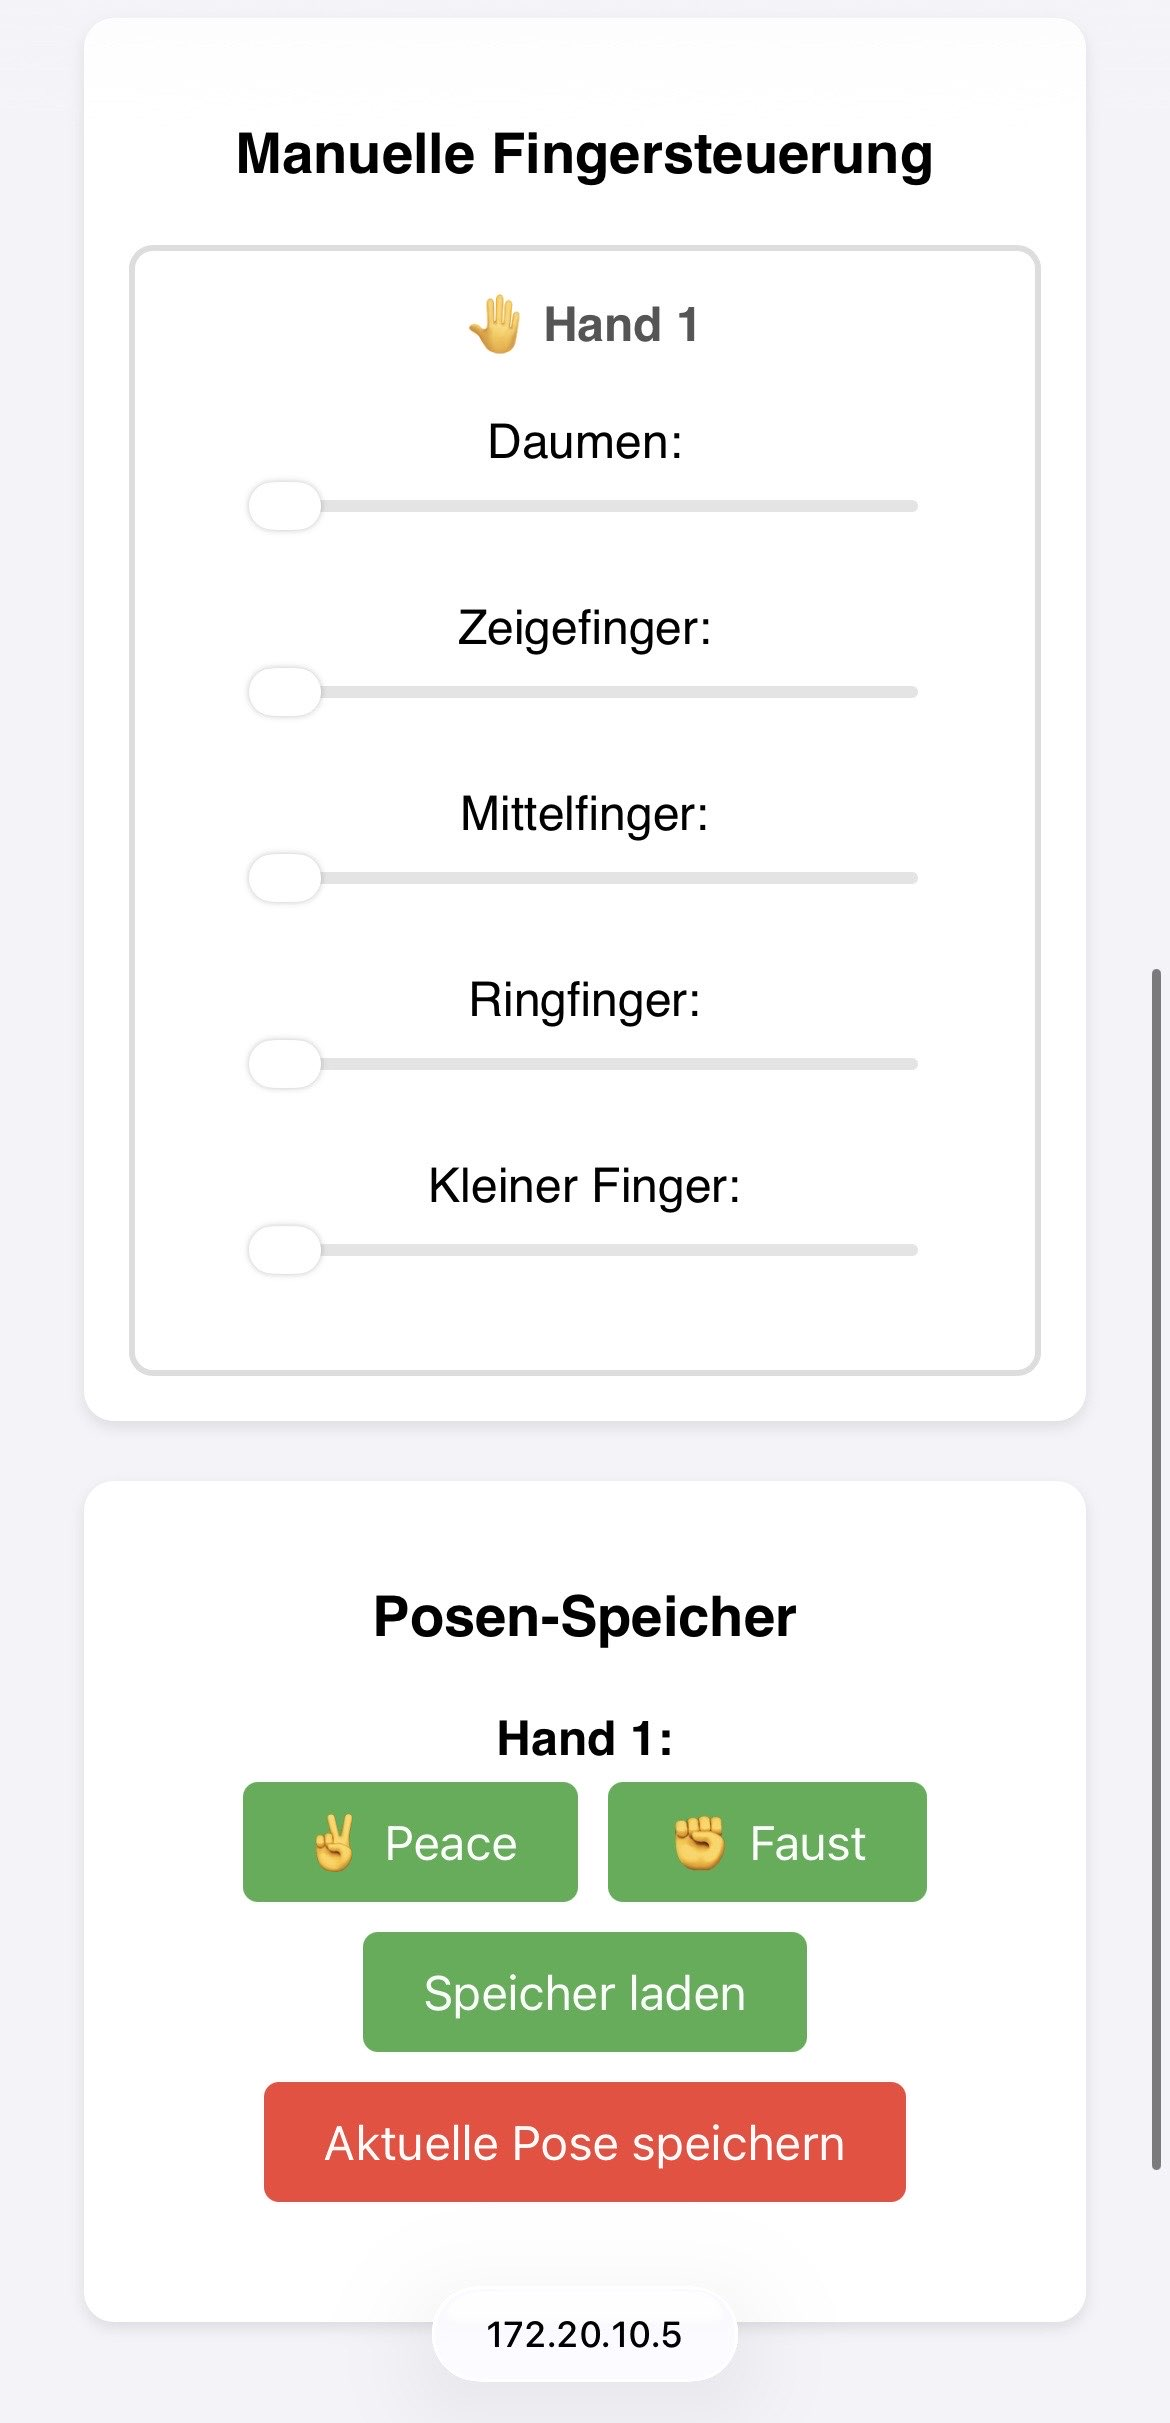
\includegraphics[width=\textwidth]{bilder/bWeb.jpg}
        \caption{Website-Steuerung auf dem Smartphone}
    \end{minipage}
\end{figure}

\newpage

\subsection{Flex-Sensor-Modus}
Im Flex-Sensor-Modus wird der Handschuh getragen und der Modus über die Website 
aktiviert. Ab diesem Zeitpunkt liest der ESP32 die fünf Flex-Sensoren aus, filtert 
die Rohwerte mit dem MedianFilter und berechnet die Änderungen per Diff-Prinzip. 
Die Servomotoren folgen den Fingerbewegungen nahezu in Echtzeit: Beim Biegen eines 
Fingers steigt der akkumulierte Differenzwert an und der zugehörige Servo bewegt 
sich in Richtung ,,geschlossen``. Beim Strecken des Fingers sinkt der Akkumulatorwert 
entsprechend und der Servo öffnet sich wieder. Die Schieberegler der Website werden 
in diesem Modus deaktiviert und ausgegraut dargestellt.

Eine Erweiterung auf zwei Hände ist grundsätzlich möglich, setzt jedoch den Aufbau 
eines zweiten Handschuhs mit fünf weiteren Flex-Sensoren voraus. Zusätzlich müssen 
im Code die analogen Eingangspins für die zweite Hand auf freie ADC1-Pins 
konfiguriert werden, da ADC2-Pins bei aktivem WLAN nicht nutzbar sind.

\subsection{Kamera-Modus}
Im Kamera-Modus wird eine separate Python-Anwendung auf einem PC gestartet, die über eine Webcam die Hand des Benutzers erfasst. MediaPipe analysiert das Kamerabild und bestimmt für jeden Finger, ob er geöffnet oder geschlossen ist. Die Erkennung basiert auf dem Vergleich der y-Koordinaten von Fingerspitze und Mittelgelenk: Liegt die Fingerspitze im Bild oberhalb des Mittelgelenks, gilt der Finger als offen (Wert 180), andernfalls als geschlossen (Wert 0). Die fünf resultierenden Werte werden als kommagetrennte Zeichenkette per USB-Serial an den ESP32 übertragen, der sie einliest, den jeweiligen Fingern zuordnet und in kalibrierte Servo-Winkel umrechnet.

Im Zwei-Hand-Modus erkennt MediaPipe beide Hände im Kamerabild gleichzeitig und überträgt zehn Werte an den ESP32, der diese den beiden Roboterhänden zuordnet. Voraussetzung ist, dass auf der Website zuvor ,,2 Hände`` ausgewählt wurde und im Code die analogen Pins sowie PCA9685-Kanäle für die zweite Hand konfiguriert sind.

\begin{figure}[H]
    \centering
    \includegraphics[width=0.7\textwidth]{bilder/eineHand.png}
    \caption{Kamera-Modus: Erkennung einer Hand}
\end{figure}

\begin{figure}[H]
    \centering
    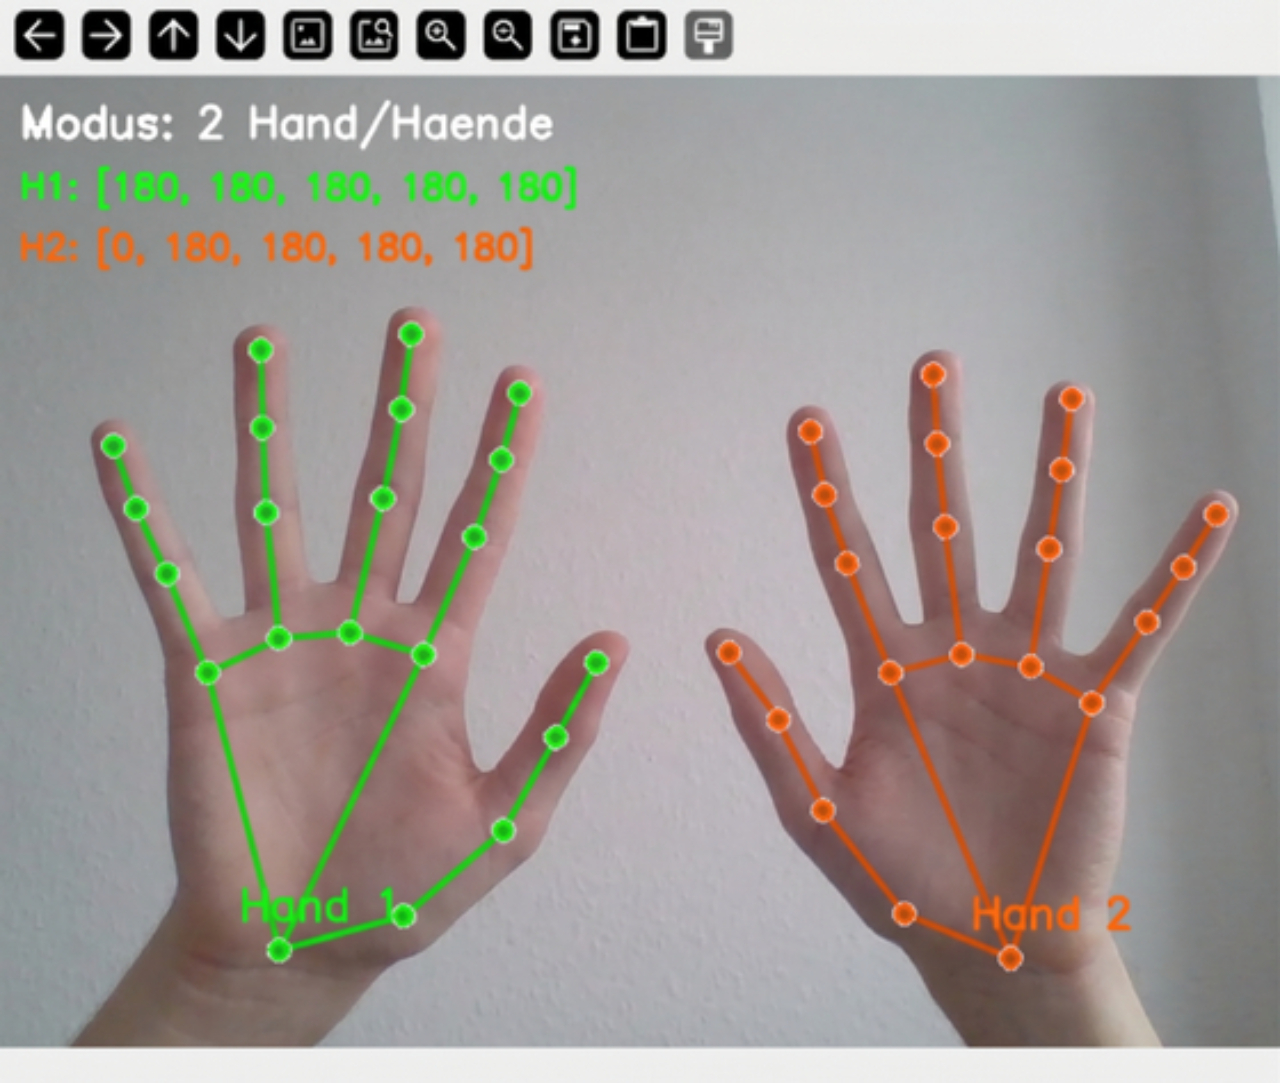
\includegraphics[width=0.7\textwidth]{bilder/zweiHaende.png}
    \caption{Kamera-Modus: Erkennung zweier Hände}
\end{figure}

% ============================================================
% 4. HARDWARE
% ============================================================
\section{Hardware}

\subsection{Komponenten}
Für die Umsetzung des Projekts wurden folgende Hardware-Komponenten eingesetzt:

\begin{table}[h]
\centering
\begin{tabular}{|l|c|l|}
\hline
\textbf{Bauteil} & \textbf{Anzahl} & \textbf{Funktion} \\
\hline
ESP32  & 1 & Mikrocontroller -- Verarbeitung, WLAN, Serial \\
PCA9685 & 1 & 16-Kanal-PWM-Treiber für Servomotoren \\
Servomotor & 5 & Steuerung je eines Fingers \\
Flex-Sensor & 5 & Messung der Fingerbiegung \\
Lithium-Batterie (3{,}7\,V) & 1 & Separate Stromversorgung der Servos \\
Widerstand (10\,k$\Omega$) & 5 & Spannungsteiler für Flex-Sensoren \\
Handschuh & 1 & Träger der Flex-Sensoren \\
D-Sub-Stecker 25-polig (w) & 1 & Steckverbinder am Handschuh (weiblich) \\
D-Sub-Stecker 25-polig (m) & 1 & Steckverbinder auf ESP32-Seite (männlich) \\
Mehradriges Kabel & 1 & Signalleitung zwischen Handschuh und Platine \\
Schrumpfschlauch & -- & Isolierung der Lötstellen an den Flex-Sensoren \\
Buchsenleiste 1$\times$8 & 3 & Steckverbindung zwischen Platine und ESP32 \\
Jumperkabel & -- & Verbindung der Komponenten \\
Platine (Lochraster) & 1 & Spannungsteiler, Widerstände und Buchsenleiste \\
\hline
\end{tabular}
\caption{Verwendete Komponenten}
\end{table}

\subsection{Funktionsweise des Flex-Sensors}

Der Flex-Sensor ist das zentrale Bauteil zur Erfassung der Fingerbewegungen. Er besteht aus einem flexiblen Substrat, auf dem eine leitfähige Tinte in einem segmentierten Muster aufgebracht ist.

\subsubsection{Aufbau}
Der Sensor setzt sich aus mehreren Schichten zusammen:
\begin{itemize}[itemsep=2pt]
    \item \textbf{Phenolharz-Substrat:} Dünne, flexible Grundlage des Sensors
    \item \textbf{Leitfähige Tinte:} Trägt den elektrischen Strom
    \item \textbf{Segmentierter Leiter:} Ermöglicht die Widerstandsänderung bei Biegung
\end{itemize}

\begin{figure}[H]
    \centering
    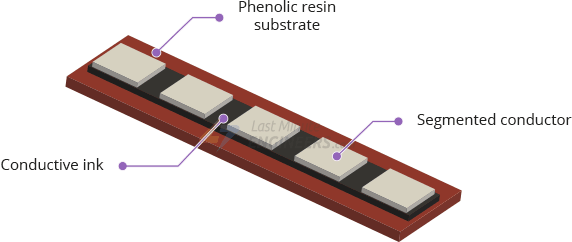
\includegraphics[width=0.7\textwidth]{bilder/Flex-Sensor-Construction.png}
    \caption{Aufbau eines Flex-Sensors (Quelle: Last Minute Engineers)}
\end{figure}

\subsubsection{Funktionsprinzip}
Im gestreckten Zustand weist der Sensor einen niedrigen elektrischen Widerstand auf (ca. 25\,k$\Omega$). Wird der Sensor gebogen, vergrößern sich die Abstände zwischen den Segmenten der leitfähigen Tinte, wodurch der Widerstand steigt. Bei einer Biegung um 45° erhöht sich der Widerstand auf etwa 62{,}5\,k$\Omega$, bei 90° auf ca. 100\,k$\Omega$.

\begin{figure}[H]
    \centering
    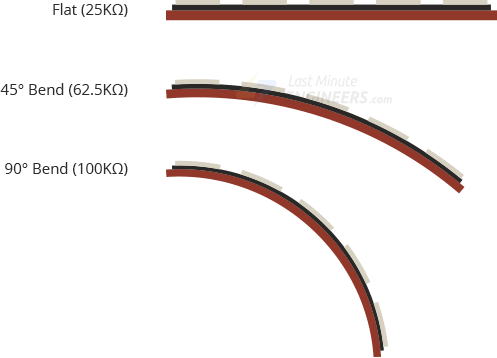
\includegraphics[width=0.7\textwidth]{bilder/Flex-Sensor-Working.png}
    \caption{Widerstandsänderung bei unterschiedlichen Biegewinkeln (Quelle: Last Minute Engineers)}
\end{figure}

Diese Widerstandsänderung wird über einen Spannungsteiler in eine messbare Spannung umgewandelt, die der ESP32 über seinen ADC (Analog-Digital-Converter) einliest. Je stärker der Finger gebeugt wird, desto höher ist der gemessene ADC-Wert.

\subsection{Schaltungsaufbau}

\begin{figure}[h]
    \centering
    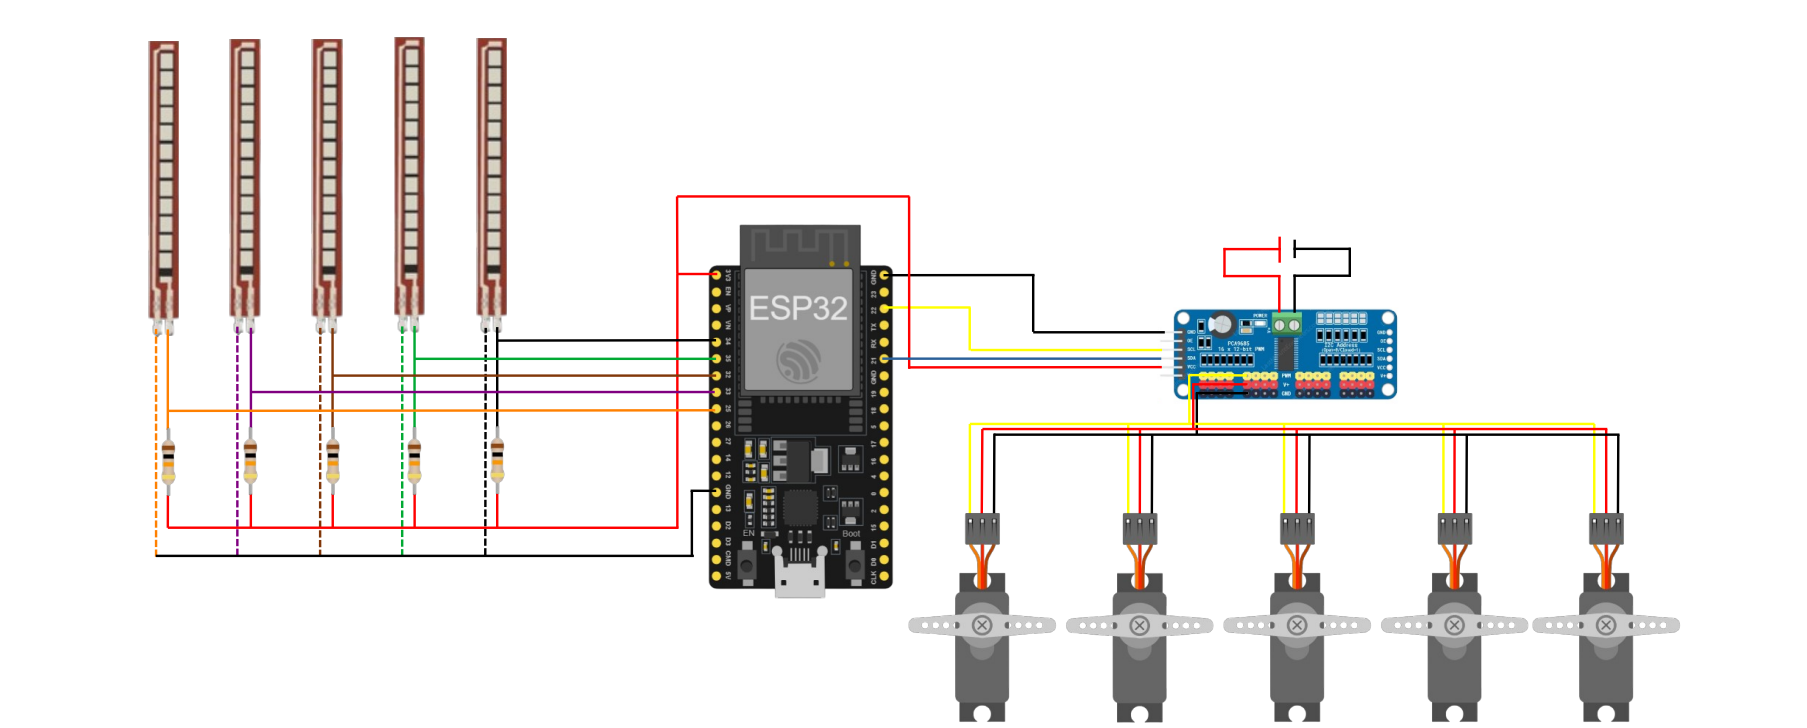
\includegraphics[width=1\textwidth]{bilder/schaltung.png}
    \caption{Schaltungsaufbau der Roboterhand}
\end{figure}

\newpage

Der ESP32 ist per I2C mit dem PCA9685 verbunden, an den die fünf Servomotoren sowie eine separate Lithium-Batterie zur Stromversorgung angeschlossen sind. Die Flex-Sensoren sind über die analogen Eingangspins des ESP32 eingebunden. Jeder Sensor bildet zusammen mit einem 10\,k$\Omega$-Widerstand einen Spannungsteiler, dessen Ausgangsspannung am jeweiligen ADC-Pin des ESP32 gemessen wird. 

Die Verbindung zwischen dem Handschuh und der Steuerelektronik erfolgt über einen 25-poligen D-Sub-Steckverbinder: Der weibliche Teil sitzt am Handschuh, der männliche auf der ESP32-Seite. Die Signalleitungen vom weiblichen Stecker führen auf eine Lochrasterplatine, auf der die Spannungsteiler aufgebaut und die Widerstände sowie eine 3$\times$8 Buchsenleiste zur Anbindung an den ESP32 verlötet sind. Aufgetretene Probleme mit der Stabilität der Kabelverbindungen am Stecker sind in Abschnitt~\ref{sec:kabel} beschrieben.

\subsection{Pinbelegungstabelle}

Bei der Auswahl der GPIO-Pins wurde darauf geachtet, dass ausschließlich Pins des ADC1 für die Flex-Sensoren verwendet werden, da ADC2 bei aktivem WLAN nicht nutzbar ist. Die folgende Tabelle gibt eine Übersicht über alle verwendeten Verbindungen:

\begin{table}[H]
\centering
\begin{tabular}{|l|l|l|}
\hline
\textbf{Komponente} & \textbf{Signal} & \textbf{ESP32-Pin} \\
\hline
PCA9685 & SDA & GPIO 21 \\
PCA9685 & SCL & GPIO 22 \\
PCA9685 & VCC & 3{,}3\,V \\
PCA9685 & GND & GND \\
\hline
Flex-Sensor 1 (Daumen)         & Analog (ADC1) & A0 -- GPIO 36 \\
Flex-Sensor 2 (Zeigefinger)    & Analog (ADC1) & A3 -- GPIO 39 \\
Flex-Sensor 3 (Mittelfinger)   & Analog (ADC1) & A6 -- GPIO 34 \\
Flex-Sensor 4 (Ringfinger)     & Analog (ADC1) & A7 -- GPIO 35 \\
Flex-Sensor 5 (Kleiner Finger) & Analog (ADC1) & A4 -- GPIO 32 \\
\hline
Servo 1 (Daumen)         & PWM (via PCA9685) & Kanal 0 \\
Servo 2 (Zeigefinger)    & PWM (via PCA9685) & Kanal 1 \\
Servo 3 (Mittelfinger)   & PWM (via PCA9685) & Kanal 2 \\
Servo 4 (Ringfinger)     & PWM (via PCA9685) & Kanal 3 \\
Servo 5 (Kleiner Finger) & PWM (via PCA9685) & Kanal 4 \\
\hline
Lithium-Batterie & VCC (Servos) & PCA9685 V+ \\
Lithium-Batterie & GND          & GND \\
\hline
\end{tabular}
\caption{Pinbelegung des ESP32}
\end{table}

\subsection{Handschuh-Konstruktion}

\subsubsection{Funktion}
Der Handschuh dient als Träger der fünf Flex-Sensoren und überträgt die 
Biegung jedes einzelnen Fingers in ein elektrisches Signal. Über einen 
abnehmbaren Steckverbinder werden die Sensorsignale an die Steuerelektronik 
weitergegeben, die daraus die Bewegungen der Roboterhand berechnet.

\subsubsection{Aufbau}
Auf jedem Finger des Handschuhs ist ein Flex-Sensor angebracht. Der untere
Teil des Sensors ist mit dem Handschuh verklebt, um eine stabile Grundlage 
zu schaffen; der Sensor ist zusätzlich aufgenäht, damit er sich bei 
Fingerbewegungen kontrolliert mitbewegt, ohne zu verrutschen. Da der 
nutzbare Messbereich der Sensoren sehr klein ist, ist eine reproduzierbare 
Positionierung am Finger entscheidend für die Qualität der Steuerung. Weitere 
Details zur Befestigung sowie aufgetretene Probleme sind in 
Abschnitt~\ref{sec:befestigung} beschrieben.

\vspace{0.5em}
\textbf{Verbindung über D-Sub-Stecker}\\
Um eine zuverlässige und lösbare Verbindung zwischen Handschuh und 
Steuerelektronik herzustellen, wurde ein 25-poliger D-Sub-Stecker 
eingesetzt. Der weibliche Teil sitzt am Handschuh und wurde mit Heißkleber 
auf der Rückseite, etwa auf Höhe des Handgelenks, befestigt. Dadurch sitzt 
der Stecker stabil und ermöglicht ein einfaches An- und Abstecken des Kabels.

\begin{figure}[H]
    \centering
    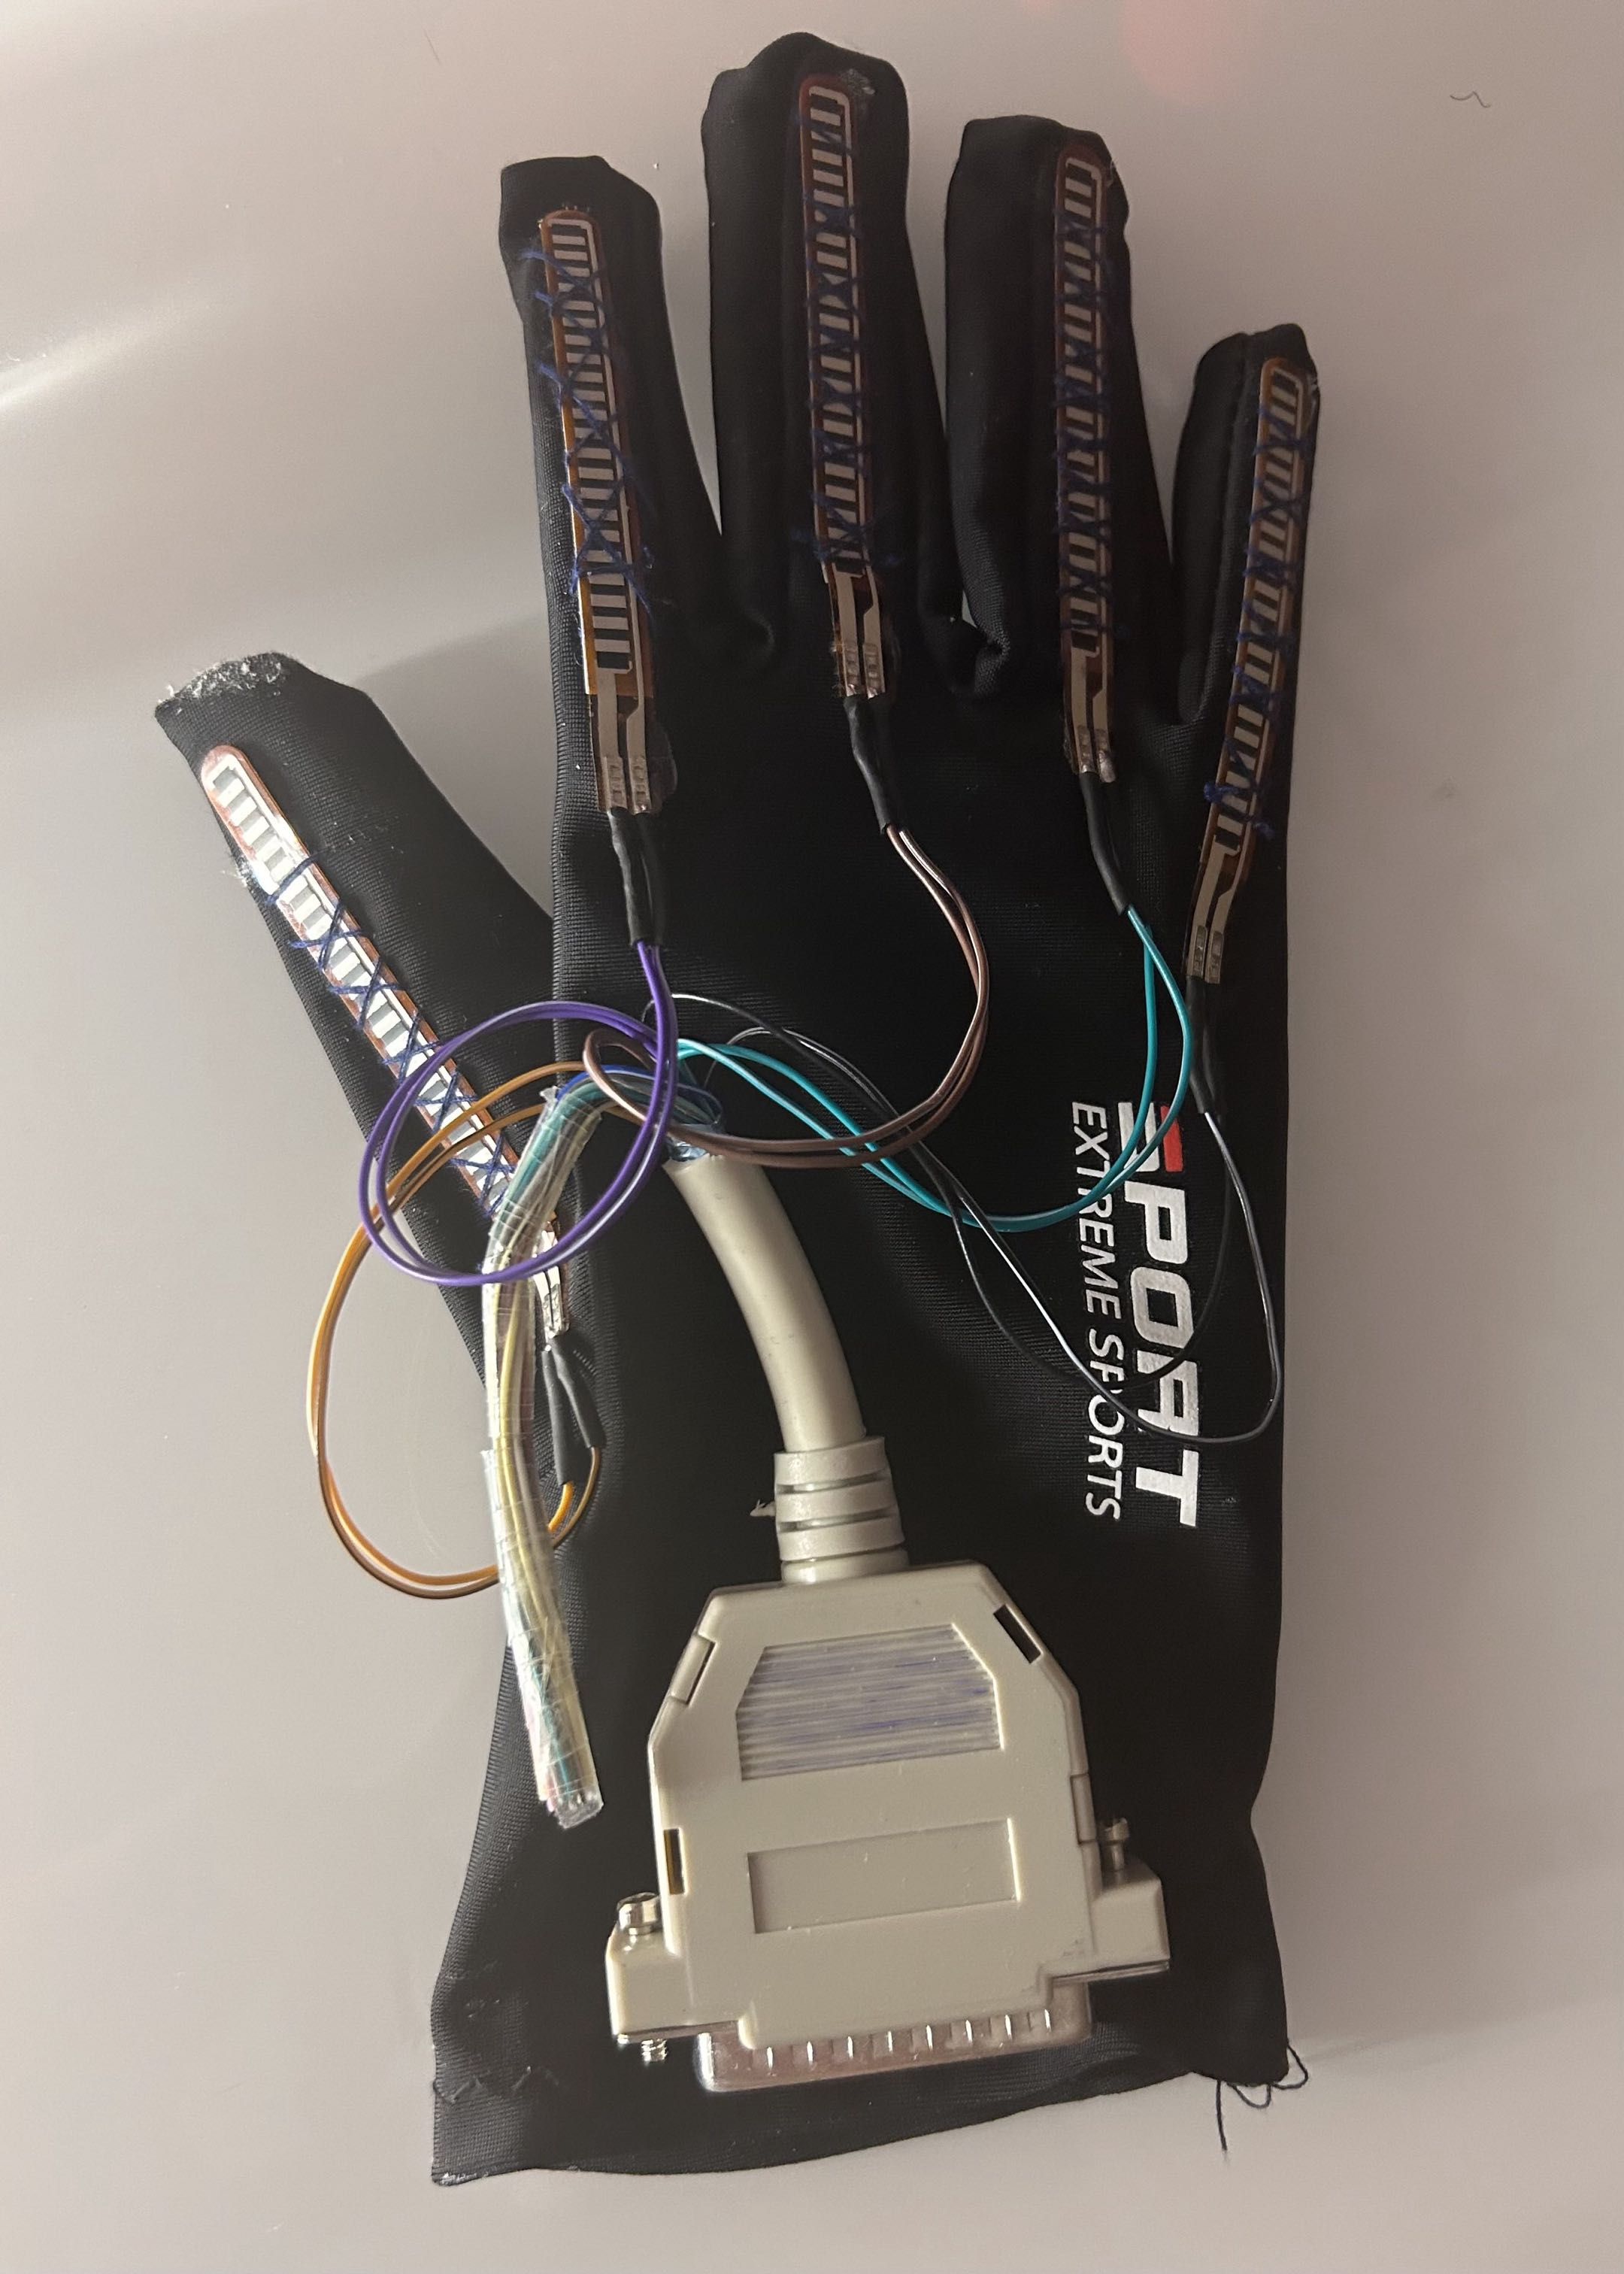
\includegraphics[width=0.3\textwidth]{bilder/Handschuh.jpg}
    \caption{Handschuh mit D-Sub-Stecker auf der Rückseite}
\end{figure}

\vspace{0.5em}

\textbf{Verkabelung am Handschuh (weibliche Seite)} \\
Für die Verdrahtung wurde ein mehradriges Kabel aufgeschnitten und die Adern 
anhand ihrer Farben den einzelnen Fingern zugeordnet. Die folgende Tabelle 
zeigt die verwendete Farbkodierung:

\begin{table}[h]
\centering
\begin{tabular}{|l|l|l|}
\hline
\textbf{Finger} & \textbf{Ader 1} & \textbf{Ader 2} \\
\hline
Daumen         & Orange          & Orange-Schwarz \\
Zeigefinger    & Lila            & Lila-Weiß      \\
Mittelfinger   & Braun           & Braun-Weiß     \\
Ringfinger     & Grün            & Grün-Weiß      \\
Kleiner Finger & Schwarz         & Schwarz-Weiß   \\
\hline
\end{tabular}
\caption{Farbkodierung der Adern für die fünf Flex-Sensoren}
\end{table}

Die jeweils zwei passenden Adern pro Finger wurden an den zugehörigen 
Flex-Sensor gelötet. Um die Lötstellen zu schützen und elektrisch zu 
isolieren, wurde über jede Verbindung ein Stück Schrumpfschlauch gezogen 
und mit einem Heißluftfön erhitzt, sodass der Schlauch eng anliegt. Die 
nicht benötigten Adern des 25-poligen Kabels wurden abgeschnitten und mit 
Heißkleber fixiert.

\vspace{0.5em}
\textbf{Verkabelung auf der ESP32-Seite (männliche Seite)} \\
Auf der anderen Seite wurde der männliche D-Sub-Stecker verwendet. Auch 
hier wurde das Kabel aufgeschnitten und die farblich passenden Adern -- 
entsprechend der obigen Zuordnung -- herausgeführt. Diese Adern wurden 
auf einer Lochrasterplatine verlötet, auf der sich auch die fünf 
10\,k$\Omega$-Widerstände für die Spannungsteiler befinden. Je eine Ader 
pro Sensor ist mit dem Signalpin verbunden, die andere mit GND. Die 
Widerstände verbinden die Signalpins mit der 3{,}3\,V-Versorgungsspannung.

Zur strukturierten Anbindung an den ESP32 ist auf der Lochrasterplatine 
eine 3$\times$8 Buchsenleiste aufgelötet. Von den 
acht Positionen werden fünf für die Flex-Sensoren genutzt. Die drei Reihen 
entsprechen den drei Signalarten: Signalpin (zum ADC des ESP32), 
Versorgungsspannung (3{,}3\,V) und GND. Die Verbindung zum ESP32 erfolgt 
über Jumperkabel, die in die Buchsenleiste gesteckt werden.

\subsubsection{Probleme und Lösungen}

Im Verlauf des Projekts traten verschiedene Herausforderungen auf, insbesondere 
bei der Befestigung der Flex-Sensoren am Handschuh sowie bei der Stabilität 
der Kabelverbindungen am D-Sub-Stecker. Eine detaillierte Beschreibung dieser 
Probleme sowie der entwickelten Lösungsansätze findet sich in Abschnitt~\ref{sec:befestigung} 
und Abschnitt~\ref{sec:kabel}.

% ============================================================
% 5. SOFTWARE
% ============================================================
\section{Software}

\subsection{Benutzte Programme}

\textbf{LibreOffice Draw} \\
LibreOffice Draw wurde zur Erstellung des Schaltplans eingesetzt. Das Programm 
ermöglicht die übersichtliche grafische Darstellung von Schaltkreisen und 
Verbindungen.

\vspace{0.5em}
\textbf{Arduino IDE (C++)} \\
Die Programmierung des ESP32 erfolgte in C++ mit der Arduino IDE. Folgende 
Bibliotheken kommen zum Einsatz:

\vspace{0.5em}
\begin{itemize}[itemsep=4pt]
    \item \textbf{Wire} \\
    Standardbibliothek für die I2C-Kommunikation. Wird für die Anbindung des 
    PCA9685-PWM-Treibers an den ESP32 verwendet.

    \item \textbf{Freenove\_4WD\_Car\_For\_ESP32} \\
    Wird zusammen mit dem Freenove-Entwicklungsboard genutzt und stellt die 
    Ansteuerung der Servomotoren sowie board-spezifische Hilfsfunktionen bereit.

    \item \textbf{WiFi} \\
    Ermöglicht die Verbindung des ESP32 mit dem lokalen WLAN, das die Grundlage 
    für die Website-Steuerung bildet.

    \item \textbf{WebServer} \\
    Stellt die HTTP-Funktionalität bereit, mit der der ESP32 die Weboberfläche 
    hostet und Steuerbefehle vom Browser entgegennimmt.

    \item \textbf{MedianFilter} \\
    Implementiert einen digitalen Filter, der aus einer Reihe aufeinanderfolgender 
    Messwerte den Median (mittleren Wert) berechnet. Im Gegensatz zum arithmetischen 
    Mittelwert ist der Median gegenüber einzelnen Ausreißern unempfindlich: Auch wenn 
    ein einzelner Messwert stark vom eigentlichen Signal abweicht, beeinflusst er das 
    Ergebnis nur minimal, da er beim Sortieren der Werte an den Rand wandert und nicht 
    in die Berechnung einfließt. Dies macht den MedianFilter besonders geeignet zur 
    Unterdrückung sporadischer Spitzen (Spikes) in Sensorsignalen, ohne die 
    Reaktionszeit merklich zu verzögern. Die Bibliothek wurde auf Empfehlung des 
    Betreuers ausgewählt und hat sich im Projekt als äußerst wirksam erwiesen.
\end{itemize}

\textbf{Visual Studio Code (Python)} \\
Die Programmierung des Python-Skripts für den KI-Kamera-Modus erfolgte in 
Visual Studio Code. Folgende Bibliotheken kommen zum Einsatz:

\vspace{0.5em}
\begin{itemize}[itemsep=4pt]
    \item \textbf{OpenCV (\texttt{cv2})} \\
    Wird für den Zugriff auf die Webcam und die Verarbeitung des Kamerabildes 
    in Echtzeit verwendet.

    \item \textbf{MediaPipe 0.10.14 (\texttt{mediapipe})} \\
    MediaPipe ist ein von Google entwickeltes Framework für maschinelles Lernen, 
    das vortrainierte Modelle zur Echtzeit-Erkennung von Gesichtern, Händen, Posen 
    und anderen visuellen Mustern bereitstellt. Für dieses Projekt wird die 
    Hands-Komponente verwendet, die 21 dreidimensionale Landmarken pro erkannter 
    Hand liefert -- von der Handwurzel über die Fingergelenke bis zu den Fingerspitzen.
    
    Im Projekt wurde gezielt die Legacy-Version 0.10.14 (\texttt{mp.solutions}) gewählt, 
    da diese durch ihre breite Dokumentationslage und den umfangreichen Community-Support 
    besser für Hardware-Projekte geeignet ist als die neuere Tasks-API. Die meisten 
    verfügbaren Tutorials und Beispiele für Robotik-Anwendungen basieren auf dieser 
    älteren API, was die Integration erheblich erleichterte.

    \item \textbf{PySerial (\texttt{serial})} \\
    Ermöglicht die serielle Kommunikation zwischen dem Python-Skript und dem 
    ESP32 über die USB-Schnittstelle.

    \item \textbf{Requests (\texttt{requests})} \\
    Wird verwendet, um den aktuellen Betriebsmodus des ESP32 per HTTP abzufragen 
    und das Skript automatisch mit der Website-Steuerung zu synchronisieren.
\end{itemize}

\vspace{0.5em}



% ============================================================
% 6. CODIERUNG UND PROBLEMLÖSUNG
% ============================================================
\subsection{Codierung und Problemlösung}

In diesem Kapitel wird die softwareseitige Umsetzung des Projekts beschrieben. Der Fokus liegt auf der Entwicklung des Flex-Sensor-Modus, der Website-Steuerung sowie des KI-Kamera-Modus.

\subsubsection{Flex-Sensor-Modus}
\vspace{0.5em}

\textbf{Entwicklung und Kalibrierung} \\
Zu Beginn wurde ein separates Testprogramm erstellt, mit dem die Servos über den Serial Monitor manuell auf beliebige Winkelwerte gesetzt werden konnten. Dadurch wurden die mechanischen Grenzen jedes Fingers ermittelt und als Konstanten im Code hinterlegt:

\begin{lstlisting}[language=C++, caption={Servo-Grenzwerte für Hand 1}]
const int servoLow[5]  = {  80,  60,  80, 115, 140 }; // offen
const int servoHigh[5] = { 120, 120, 120,  70,  70 }; // geschlossen
\end{lstlisting}

Anschließend wurde ein erster Flex-Sensor eingebunden: Der analoge Eingabewert wird über den Serial Monitor ausgelesen, über \texttt{map()} in den entsprechenden Servo-Winkel umgerechnet und mit \texttt{constrain()} auf den zulässigen Bereich begrenzt. Nach erfolgreicher Validierung mit einem Sensor wurde der Code auf alle fünf Finger ausgeweitet.

\vspace{0.5em}
Bei den ersten Tests zeigte sich, dass die Sensoren unregelmäßige Spitzen (Spikes) lieferten, die zu ruckartigen Bewegungen der Servos führten.

\textbf{Mittelwert-Filter (erster Ansatz)} \\
Als erster Lösungsansatz wurden die letzten sechs Messwerte gemittelt. Dies reduzierte die Ausreißer deutlich, verursachte jedoch eine merkliche Verzögerung, da Extremwerte in den Mittelwert einfließen.

\vspace{0.5em}
\textbf{MedianFilter (zweiter Ansatz)} \\
Nach einem Gespräch mit dem Lehrer wurde die \textit{MedianFilter}-Bibliothek auf GitHub empfohlen. Die Bibliothek speichert die letzten Messwerte in einem Puffer und gibt bei jeder Abfrage den mittleren Wert zurück. Da der Median gegenüber Extremwerten robuster ist als der arithmetische Mittelwert, werden Spikes zuverlässiger herausgefiltert, ohne die Reaktionszeit zu erhöhen. Für das Projekt wurden 15 Pufferwerte gewählt, mit einem Startwert nahe dem typischen Ruhewert jedes Sensors:

\begin{lstlisting}[language=C++, caption={Initialisierung der MedianFilter für alle fünf Finger}]
MedianFilter flexFilter0(15, 3200);
MedianFilter flexFilter1(15, 3170);
MedianFilter flexFilter2(15, 3170);
MedianFilter flexFilter3(15, 3170);
MedianFilter flexFilter4(15, 3040);

MedianFilter* flexFilters[5] = {
  &flexFilter0, &flexFilter1, &flexFilter2,
  &flexFilter3, &flexFilter4
};
\end{lstlisting}

Die Funktion \texttt{leseFlex()} liest jeden Sensor aus und schickt den Rohwert durch den zugehörigen Filter:

\begin{lstlisting}[language=C++, caption={Funktion leseFlex() -- Rohwert einlesen und filtern}]
void leseFlex() {
  for (int i = 0; i < 5; i++) {
    roheWerte[i]   = analogRead(flexPins[i]);
    saubereWerte[i] = flexFilters[i]->in(roheWerte[i]);
  }
  if (numHaende == 2) {
    for (int i = 0; i < 5; i++) {
      roheWerte2[i]   = analogRead(flexPins2[i]);
      saubereWerte2[i] = flexFilters2[i]->in(roheWerte2[i]);
    }
  }
}
\end{lstlisting}

\newpage

\textbf{Problem: }Die minimalen und maximalen Messwerte der Flex-Sensoren sind instabil – sie verändern sich durch Temperatur sowie durch Fingerbewegungen selbst. Dies führt zu Fehlinterpretationen und erfordert eine manuelle Neukalibrierung (eine genauere Beschreibung folgt in Abschnitt~\ref{sec:drift}).

\vspace{0.5em}
\textbf{Diff-Prinzip (finale Lösung)} \\
Da das Problem nicht das Rauschen, sondern die Unzuverlässigkeit der Absolutwerte war, wurde ein Ansatz gesucht, der ohne feste Grenzwerte auskommt. Die Kernidee: Nur die \textit{Änderung} des Sensorwerts wird ausgewertet, nicht der Wert selbst. Pro Messzyklus wird die Differenz zum letzten Wert berechnet, zu einem internen Akkumulator addiert und auf den Servo-Winkel gemappt:

\begin{lstlisting}[language=C++, caption={Diff-Prinzip in der Hauptschleife (Hand 1)}]
for (int i = 0; i < 5; i++) {
  int diff     = saubereWerte[i] - lastWerte[i];
  lastWerte[i] = saubereWerte[i];
  wertDiff[i]  = constrain(wertDiff[i] + diff, diffMin[i], diffMax[i]);
  int servoZiel = map(wertDiff[i], diffMin[i], diffMax[i],
                      servoLow[i], servoHigh[i]);
  aktuelleWerte[i] = servoZiel;
  Servo_Angle(servoPins[i], servoZiel);
}
\end{lstlisting}

Da das System ausschließlich auf \textit{Veränderungen} reagiert, spielt der absolute Grundwert keine Rolle mehr -- ob der Sensor bei 3180 oder 3200 liegt, der Servo bewegt sich nur bei einer tatsächlichen Biegeänderung. Der einzige verbleibende Tuning-Parameter ist der Akkumulatorbereich (\texttt{diffMax}): Ein kleinerer Wert macht die Hand empfindlicher, ein größerer erfordert stärkere Bewegungen für den vollen Servo-Ausschlag. Manuelle Kalibrierungen sind damit dauerhaft überflüssig.

\newpage

\subsubsection{Website-Steuerung}

Der ESP32 hostet eine Weboberfläche, die über dessen IP-Adresse im lokalen Netzwerk per Browser erreichbar ist. Die Oberfläche ist in vier funktionale Bereiche unterteilt und wird vollständig als HTML-String im C++-Code erzeugt und direkt vom ESP32 ausgeliefert.

\vspace{0.5em}
\textbf{Moduswechsel und Handanzahl} \\
Der aktuelle Betriebsmodus wird serverseitig als globale Variable gespeichert. Klickt der Benutzer auf der Website einen Modus-Button, sendet der Browser eine HTTP-Anfrage an den Handler \texttt{/setMode}. Dieser setzt die Variable und -- falls auf Flex-Modus gewechselt wird -- setzt auch alle Diff-Akkumulatoren zurück, damit die Hand in einer definierten Ausgangsposition startet:

\begin{lstlisting}[language=C++, caption={Handler: Moduswechsel und Reset der Diff-Akkumulatoren}]
void handleSetMode() {
  String val = server.arg("val");
  if      (val == "manual") aktuellerModus = MODE_MANUAL;
  else if (val == "flex")   aktuellerModus = MODE_FLEX;
  else if (val == "camera") aktuellerModus = MODE_CAMERA;

  if (val == "flex") {
    for (int i = 0; i < 5; i++) {
      wertDiff[i]  = 0;  lastWerte[i]  = 0;
      wertDiff2[i] = 0;  lastWerte2[i] = 0;
    }
  }
  server.send(200, "text/plain", "OK");
}
\end{lstlisting}

\vspace{0.5em}
\textbf{Schieberegler und Servo-Steuerung} \\
Bewegt der Benutzer einen Schieberegler, sendet die Website den Wert (0--180) über \texttt{/setServo} an den ESP32. Der Handler prüft, ob Website-Modus aktiv ist, und mappt den Schieberwert auf den mechanischen Bereich des jeweiligen Servos. Jeder Finger hat dabei eigene Grenzwerte, da die Servos unterschiedlich verbaut sind:

\begin{lstlisting}[language=C++, caption={Handler: Schieberegler-Wert auf Servo-Winkel mappen}]
void handleSetServo() {
  if (aktuellerModus != MODE_MANUAL) {
    server.send(200, "text/plain", "OK"); return;
  }
  int hand = server.arg("hand").toInt();
  int id   = server.arg("id").toInt();
  int val  = server.arg("val").toInt();

  int mapped = val;
  if (hand == 1) {
    aktuelleWerte[id] = val;
    if (id == 0) mapped = map(val, 0, 180,  80, 120);
    if (id == 1) mapped = map(val, 0, 180,  60, 120);
    if (id == 2) mapped = map(val, 0, 180,  80, 120);
    if (id == 3) mapped = map(val, 0, 180, 115,  70);
    if (id == 4) mapped = map(val, 0, 180, 140,  70);
    Servo_Angle(servoPins[id], mapped);
  }
  // Hand 2 analog ...
  server.send(200, "text/plain", "OK");
}
\end{lstlisting}

\vspace{0.5em}
\textbf{Posenverwaltung} \\
Für die Posen ,,Peace`` und ,,Faust`` sind feste Winkelkombinationen im Code hinterlegt. Zusätzlich kann der Benutzer die aktuelle Stellung als eigene Pose speichern und später wieder abrufen. Der Handler unterscheidet zwischen \texttt{save}, \texttt{load}, \texttt{peace} und \texttt{fist} und arbeitet für beide Hände über denselben Codepfad, indem er die passenden Arrays per Pointer auswählt:

\begin{lstlisting}[language=C++, caption={Handler: Posen speichern und abrufen}]
void handleSetPose() {
  int    hand  = server.arg("hand").toInt();
  String type  = server.arg("type");

  int* werte   = (hand == 1) ? aktuelleWerte  : aktuelleWerte2;
  int* pins    = (hand == 1) ? servoPins      : servoPins2;
  int* gespeic = (hand == 1) ? gespeichertePose : gespeichertePose2;

  if (type == "save") {
    for (int i = 0; i < 5; i++) gespeic[i] = werte[i];
  } else if (aktuellerModus == MODE_MANUAL) {
    if (type == "peace") {
      int p[] = { 120, 60, 80, 115, 140 };
      for (int i = 0; i < 5; i++) {
        werte[i] = p[i]; Servo_Angle(pins[i], p[i]);
      }
    } else if (type == "fist") {
      int p[] = { 120, 120, 120, 70, 70 };
      for (int i = 0; i < 5; i++) {
        werte[i] = p[i]; Servo_Angle(pins[i], p[i]);
      }
    } else if (type == "load") {
      for (int i = 0; i < 5; i++) {
        werte[i] = gespeic[i]; Servo_Angle(pins[i], werte[i]);
      }
    }
  }
  server.send(200, "text/plain", "OK");
}
\end{lstlisting}

\vspace{0.5em}
\textbf{Dynamische Zwei-Hand-Anzeige} \\
Die Oberfläche passt sich per JavaScript dynamisch an die gewählte Handanzahl an. Wird ,,2 Hände`` ausgewählt, werden die Schieberegler und Posen-Buttons für Hand~2 eingeblendet; bei ,,1 Hand`` bleiben sie ausgeblendet. Die Auswahl wird gleichzeitig per HTTP an den ESP32 übermittelt:

\begin{lstlisting}[language=C++, caption={JavaScript auf der Website: Hand-2-Bereiche ein-/ausblenden}]
function updateUI() {
  const h2 = document.getElementById('hand2sliders');
  const p2 = document.getElementById('pose2block');
  const show2 = (numHaende === 2);
  if (h2) h2.style.display = show2 ? '' : 'none';
  if (p2) p2.style.display = show2 ? '' : 'none';
}
function setHands(n) {
  numHaende = n;
  fetch('/setHands?val=' + n);
  updateUI();
}
\end{lstlisting}

\subsubsection{KI-Kamera-Modus}

Die Kamerasteuerung basiert auf der \textit{MediaPipe}-Bibliothek und wurde als eigenständige Python-Datei entwickelt, getrennt vom ESP32-Code. Zunächst wurde die Handerkennung isoliert getestet: Die erkannten Fingerpositionen wurden im Terminal ausgegeben und auf Korrektheit geprüft, bevor die serielle Kommunikation zum ESP32 hinzugefügt wurde.

\vspace{0.5em}
\textbf{Wahl der MediaPipe-Version} \\
Für die Umsetzung wurde die ältere Legacy-API (\texttt{mp.solutions}, Version 0.10.14) verwendet, da die meisten verfügbaren Tutorials und Community-Ressourcen für Hardware-Projekte auf dieser Version basieren. Die neuere Tasks-API bietet zwar schnellere Modelle, jedoch stellt die mechanische Reaktionsgeschwindigkeit der Servomotoren den eigentlichen Flaschenhals des Systems dar, sodass eine höhere KI-Verarbeitungsgeschwindigkeit keinen messbaren Vorteil gebracht hätte.

Die Initialisierung richtet sich automatisch nach der Konfigurationsvariable \texttt{NUM\_HAENDE}:

\begin{lstlisting}[language=Python, caption={Initialisierung von MediaPipe und Webcam}]
hand_detector = mp_hands.Hands(
    max_num_hands            = NUM_HAENDE,
    min_detection_confidence = 0.7,
    min_tracking_confidence  = 0.5
)
cap = cv2.VideoCapture(0)
cap.set(cv2.CAP_PROP_FRAME_WIDTH,  640)
cap.set(cv2.CAP_PROP_FRAME_HEIGHT, 480)
\end{lstlisting}

\vspace{0.5em}
\textbf{Erkennung der Fingerzustände} \\
Die Erkennung basiert auf den 21 Landmarken, die MediaPipe pro Hand zurückgibt. Für die vier langen Finger wird die y-Koordinate der Fingerspitze mit der des Mittelgelenks verglichen -- liegt die Spitze höher im Bild, ist der Finger gestreckt. Der Daumen wird über die x-Koordinate ausgewertet, da er sich seitwärts bewegt:

\begin{lstlisting}[language=Python, caption={Funktion berechne\_winkel() -- Offen/Zu-Klassifikation aller 5 Finger}]
def berechne_winkel(lm):
    angles = []

    # Daumen: seitwaerts -> X-Koordinate
    if lm[4].x > lm[2].x:
        angles.append(180)  # offen
    else:
        angles.append(0)    # geschlossen

    # Zeige-, Mittel-, Ring-, Kleiner Finger: Y-Koordinate
    finger_tips   = [8, 12, 16, 20]
    finger_joints = [6, 10, 14, 18]
    for i in range(4):
        if lm[finger_tips[i]].y < lm[finger_joints[i]].y:
            angles.append(180)  # Spitze hoeher als Gelenk -> offen
        else:
            angles.append(0)    # geschlossen
    return angles
\end{lstlisting}

Diese binäre Auswertung (0 oder 180) ist bewusst einfach gehalten -- das Ziel war, den Modus grundsätzlich zum Laufen zu bringen, nicht eine präzise Winkelschätzung zu erzielen.

\vspace{0.5em}
\textbf{Serielle Datenübertragung} \\
Die berechneten Winkelwerte werden als kommagetrennte Zeichenkette per USB-Serial an den ESP32 gesendet. Das Format unterscheidet sich je nach Handanzahl -- bei zwei Händen werden alle zehn Werte in einer einzigen Zeile übertragen:

\begin{lstlisting}[language=Python, caption={Daten senden: Format für 1 oder 2 Hände}]
if NUM_HAENDE == 1 or angles_hand2 is None:
    # Format: "v0,v1,v2,v3,v4\n"
    data_string = "{},{},{},{},{}\n".format(*angles_hand1)
else:
    # Format: "v0,v1,v2,v3,v4,v5,v6,v7,v8,v9\n"
    data_string = "{},{},{},{},{},{},{},{},{},{}\n".format(
        *angles_hand1, *angles_hand2
    )
esp32.write(data_string.encode('utf-8'))
\end{lstlisting}

\vspace{0.5em}
\textbf{Empfang und Verarbeitung auf dem ESP32} \\
Der ESP32 liest die empfangene Zeichenkette im Kamera-Modus zeilenweise ein, zählt die Kommata und teilt die Werte entsprechend auf beide Hände auf. Anschließend werden die Werte (0 oder 180) auf die mechanischen Servo-Grenzwerte gemappt:

\begin{lstlisting}[language=C++, caption={ESP32: Serielle Daten einlesen und Servos ansteuern}]
if (aktuellerModus == MODE_CAMERA) {
  if (Serial.available() > 0) {
    String data = Serial.readStringUntil('\n');
    data.trim();

    // Kommata zaehlen und Positionen merken
    int commas[9]; int count = 0;
    for (int c = 0; c < data.length() && count < 9; c++)
      if (data[c] == ',') commas[count++] = c;

    if (count >= 4) {
      // Hand 1: erste 5 Werte extrahieren und mappen
      int v[5];
      v[0] = data.substring(0, commas[0]).toInt();
      // ... weitere Werte analog ...
      v[0] = map(v[0], 0, 180, 120, 80);
      // ... weitere Mappings analog ...
      for (int i = 0; i < 5; i++) Servo_Angle(servoPins[i], v[i]);

      // Hand 2: nur wenn 2-Hand-Modus und 10 Werte empfangen
      if (numHaende == 2 && count >= 9) {
        // Werte ab commas[4] extrahieren und mappen
      }
    }
  }
}
\end{lstlisting}

Die Zwei-Hand-Erweiterung ist damit nahtlos integriert: Das Python-Skript sendet automatisch mehr Daten, wenn \texttt{NUM\_HAENDE = 2} gesetzt ist, und der ESP32 verarbeitet sie ohne zusätzliche Handshake-Logik.

\newpage

% ============================================================
% 6. FEHLERSUCHE UND PROBLEMLÖSUNG
% ============================================================
\section{Fehlersuche und Problemlösung}

Während der Umsetzung des Projekts traten verschiedene Probleme auf, die im Rahmen der Fehlersuche analysiert und schrittweise behoben wurden. Die Lösungsansätze basierten sowohl auf eigener Analyse als auch auf Recherche und der Nutzung externer Informationsquellen. Die folgenden Abschnitte beschreiben die wichtigsten aufgetretenen Probleme, deren Ursachen sowie die getroffenen Maßnahmen.

\subsection{Spikes bei den Flex-Sensoren}

\textbf{Problem:} Die Flex-Sensoren lieferten unregelmäßige Spitzen (Spikes), die nicht der tatsächlichen Fingerbewegung entsprachen. Die Servos führten dadurch ruckartige, unkontrollierte Bewegungen aus, die eine zuverlässige Steuerung unmöglich machten.

\textbf{Ursache:} Flex-Sensoren sind analoge Bauteile, deren Signal von Natur aus mit Rauschen behaftet ist. Zusätzlich können minimale mechanische Vibrationen oder Kontaktprobleme an den Kabelverbindungen kurzfristige Ausreißer im ADC-Wert verursachen, die nicht mit einer tatsächlichen Biegebewegung des Fingers zusammenhängen.

\textbf{Lösung:} Als erster Ansatz wurde ein gleitender Mittelwert über die letzten sechs Messwerte berechnet. Dies reduzierte die Ausreißer zwar deutlich, führte jedoch zu einer spürbaren Verzögerung in der Übertragung. Daraufhin wurde der \textit{MedianFilter} implementiert, der das Delay beseitigte und die Bewegungen erheblich gleichmäßiger und präziser machte, da der Median gegenüber Extremwerten robuster ist als der arithmetische Mittelwert.

\subsection{Drift der Flex-Sensor-Werte durch Temperatur}
\label{sec:drift}

\textbf{Problem:} Die Flex-Sensoren weisen einen sehr kleinen Messbereich auf -- der Unterschied im ADC-Rohwert zwischen vollständig gestrecktem und vollständig gebogenem Finger beträgt lediglich etwa 20 Bit. Zusätzlich driften die Absolutwerte in Abhängigkeit von Umgebungs- und Körpertemperatur. So konnte der Wert für ,,offen``, der anfangs bei 3180 lag, nach einigen Betriebsminuten auf 3200 ansteigen, wodurch die Hand eine falsche Position einnahm, obwohl keine Handbewegung stattgefunden hatte. Die Min/Max-Werte im Code mussten daraufhin jedes Mal manuell neu abgelesen und angepasst werden.

\textbf{Lösung:} Zur dauerhaften Behebung dieses Problems wurde das \textit{Diff-Prinzip} entwickelt. Statt mit Absolutwerten zu arbeiten, wird ausschließlich die relative Änderung zwischen zwei aufeinanderfolgenden Messwerten ausgewertet und akkumuliert. Da das System dadurch temperaturunabhängig arbeitet, sind manuelle Kalibrierungen nicht mehr erforderlich. Eine detaillierte Beschreibung des Verfahrens findet sich in Abschnitt~5.3.1.

\newpage

\subsection{Analoger Pin liefert konstant den Wert null}

\textbf{Problem:} In der ursprünglichen Pinbelegung wurde für den kleinen Finger der analoge Pin GPIO 25 verwendet. Sobald das WLAN aktiv war, lieferte dieser Pin konstant den Wert 0, obwohl der Sensor korrekt angeschlossen war.

\textbf{Ursache:} Der ESP32 verfügt über zwei ADC-Einheiten: ADC1 und ADC2. ADC2 teilt intern denselben Hardware-Kanal mit dem WLAN-Treiber des Espressif-Systems. Laut offizieller Espressif-Dokumentation kann ADC2 daher nicht genutzt werden, solange WLAN aktiv ist -- der Zugriff wird blockiert und liefert als Ergebnis konstant den Wert 0. Da GPIO 25 zu ADC2 gehört, ist dieser Pin bei laufendem WLAN nicht als analoger Eingang nutzbar. Dieses Problem ist in der Dokumentation des ESP32 zwar erwähnt, wird jedoch in vielen Tutorials nicht thematisiert.

\textbf{Lösung:} Alle Flex-Sensoren wurden auf Pins des ADC1 umverdrahtet (A0, A3, A6, A7, A4 -- entspricht GPIO 36, 39, 34, 35, 32), da ADC1 vom WLAN-Treiber nicht beansprucht wird und uneingeschränkt genutzt werden kann.

\subsection{Befestigung der Flex-Sensoren am Handschuh}
\label{sec:befestigung}

\textbf{Problem:} Das zuverlässige Befestigen der Sensoren am Handschuh erwies sich als schwierig. Eine 3D-gedruckte Fingerführung aus PLA wurde konstruiert und getestet, hielt jedoch unter Belastung nicht zuverlässig und übte beim Beugen des Fingers mechanischen Druck auf den Sensor aus. Da der nutzbare Messbereich der Sensoren so klein ist, verfälschte bereits geringer Fremdeinfluss die gemessenen Werte spürbar. Außerdem zeigte sich, dass die Positionierung des Sensors am Finger sehr genau reproduzierbar sein muss -- bereits geringfügige Abweichungen in der Trageposition des Handschuhs führten zu leicht unterschiedlichen Messwerten.

\textbf{Erster Lösungsansatz: 3D-gedruckte Fingerführung} \\
Die Befestigung der Flex-Sensoren am Handschuh stellte sich im Verlauf 
des Projekts als eine der größeren praktischen Herausforderungen heraus. 
Zunächst wurde versucht, die Sensoren lediglich zu fixieren, wobei die 
Halterung am Finger nicht ausreichend stabil war. Als erster Lösungsansatz 
wurde eine 3D-gedruckte Fingerführung entwickelt und getestet. Diese 
sollte auf die einzelnen Finger geklebt werden, sodass die Sensoren 
seitlich eingeschoben werden können und dabei genug Spielraum zum Biegen 
behalten.

\begin{figure}[H]
\centering
\begin{minipage}[t]{0.48\textwidth}
    \centering
    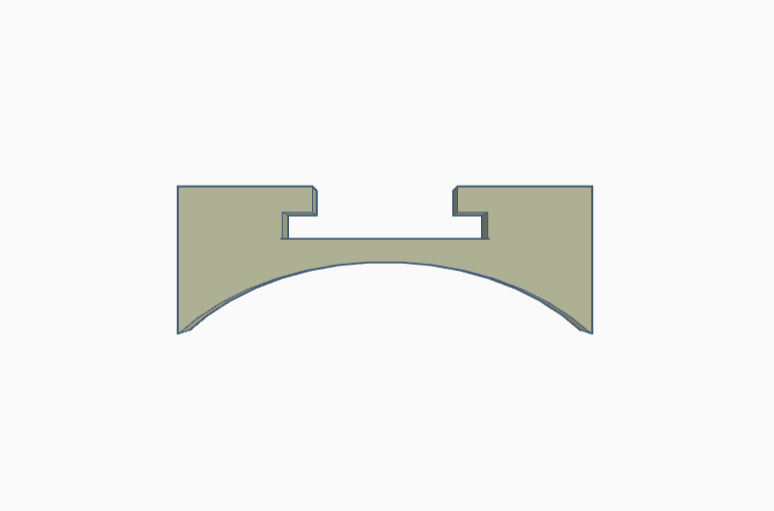
\includegraphics[width=\textwidth]{bilder/FingerFührungOben.png}
    \caption{Ansicht der Fingerführung von oben}
\end{minipage}
\hfill
\begin{minipage}[t]{0.48\textwidth}
    \centering
    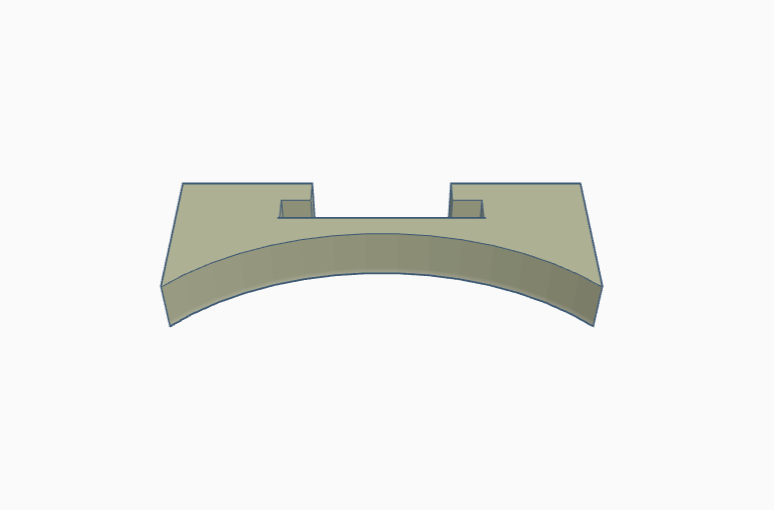
\includegraphics[width=\textwidth]{bilder/FingerFührungSeite.png}
    \caption{Ansicht der Fingerführung von der Seite}
\end{minipage}
\end{figure}

Die 3D-gedruckte Lösung erwies sich jedoch als nicht geeignet: Beim Biegen 
des Fingers wurde nicht genügend Druck auf den Sensor übertragen, sodass 
die Messwerte ungenau blieben. 

\textbf{Finale Lösung:} \\
Der untere Teil jedes Sensors wurde mit dem Handschuh verklebt und der obere Teil zusätzlich genäht. Bei einzelnen Sensoren wurde auch der obere Teil verklebt, wenn die Messwerte nicht präzise genug erschienen. Diese Kombination aus Kleben und Nähen gewährleistet sowohl die notwendige Stabilität als auch die erforderliche Flexibilität, damit der Sensor die Biegung des Fingers korrekt erfassen kann, ohne durch die Befestigung beeinflusst zu werden.

\subsection{Gleichzeitiger Zugriff auf den seriellen Port}

\textbf{Problem:} Beim Starten des Python-Skripts für den Kamera-Modus trat eine Fehlermeldung auf, die den Aufbau der seriellen Verbindung zum ESP32 verhinderte. Das Skript konnte den COM-Port nicht öffnen, obwohl der ESP32 korrekt angeschlossen war.

\textbf{Ursache:} Die Arduino IDE und das Python-Skript greifen beide über denselben seriellen COM-Port auf den ESP32 zu. Ist in der Arduino IDE der Serial Monitor geöffnet oder eine aktive Verbindung zum Board aufgebaut, belegt sie den Port exklusiv. Das Python-Skript kann diesen Port dann nicht gleichzeitig öffnen und gibt eine Fehlermeldung aus.

\textbf{Lösung:} Vor dem Start des Python-Skripts muss die serielle Verbindung in der Arduino IDE getrennt werden -- entweder durch Schließen des Serial Monitors oder durch vollständiges Beenden der Arduino IDE. Nach dem Start des Python-Skripts kann die Arduino IDE bei Bedarf wieder geöffnet werden, sofern der Serial Monitor nicht aktiviert wird.

\subsection{MediaPipe-Versionskonflikt}

\textbf{Problem:} Der Code aus verfügbaren Tutorial-Videos war für eine ältere MediaPipe-Version geschrieben und ließ sich mit der aktuell installierten Version nicht ausführen. Die Klassen- und Methodennamen hatten sich in der neueren API geändert, sodass bekannte Aufrufe zu Fehlern führten.

\textbf{Lösung:} Nach Rücksprache mit dem KI-Tool Gemini wurde entschieden, die ältere Legacy-API (\texttt{mp.solutions}, Version 0.10.14) explizit zu installieren, da diese für Hardware-Projekte besser dokumentiert ist und über einen breiteren Community-Support verfügt. Die Version wurde im Python-Environment fest fixiert, um künftige Inkompatibilitäten durch automatische Updates zu vermeiden.

\subsection{Abreißende Kabel am D-Sub-Stecker}
\label{sec:kabel}

\textbf{Problem:} Beim Tragen und Anstecken des Handschuhs rissen die direkt am D-Sub-Stecker verlöteten Kabel wiederholt an den Lötstellen ab. Durch die Zug- und Biegebeanspruchung beim Handling des Steckers wirkte die mechanische Kraft unmittelbar auf die Lötstellen, die dieser Belastung auf Dauer nicht standhielten.

\textbf{Ursache:} Lötstellen sind elektrisch zuverlässig, aber mechanisch empfindlich. Ohne zusätzliche Zugentlastung überträgt sich jede Bewegung des Kabels direkt auf die Verbindungsstelle zwischen Draht und Lötpad. Gerade an Steckverbindern, die regelmäßig ein- und ausgesteckt werden, entsteht dabei eine erhebliche Wechselbelastung.

\textbf{Lösung:} Die Lötstellen auf beiden Seiten des D-Sub-Steckers wurden großzügig mit \textbf{Heißkleber} versiegelt. Der Kleber fixiert die Kabel mechanisch direkt am Steckergehäuse und übernimmt damit die Funktion einer Zugentlastung: Zug- und Biegekräfte werden vom Kleber aufgenommen und nicht mehr an die Lötstellen weitergegeben. Die Verbindung blieb seither auch bei wiederholtem Anstecken stabil.

\newpage

% ============================================================
% 7. TESTERGEBNISSE
% ============================================================
\section{Testergebnisse}

Im Rahmen des Projekts wurden verschiedene Tests durchgeführt, um die Funktionsfähigkeit und Zuverlässigkeit der einzelnen Modi zu überprüfen. Die Tests erfolgten zunächst komponentenweise und anschließend im Gesamtbetrieb.

\subsection{Flex-Sensor-Modus}

Nach der Implementierung des Diff-Prinzips reagieren alle fünf Finger 
grundsätzlich auf Biegebewegungen, und die Übertragung erfolgt ohne 
spürbare Verzögerung. Beim Start des Modus befinden sich alle 
Akkumulatorwerte bei null, sodass die Roboterhand zunächst in der 
offenen Ausgangsposition verbleibt und erst durch aktive Fingerbewegung 
gesteuert wird. Der temperaturbedingte Drift, der bei der absoluten 
Auswertung zuvor das Hauptproblem dargestellt hatte, tritt durch das 
Diff-Prinzip nicht mehr auf.

\textbf{Beobachtetes Problem: Schleichendes Zurückdriften bei gehaltener 
Position.} Im Verlauf der Tests zeigte sich jedoch ein weiteres 
Verhalten, das in der ursprünglichen Auslegung des Diff-Prinzips nicht 
berücksichtigt wurde. Werden die Finger gebeugt und in dieser Stellung 
ruhig gehalten, bleibt die Roboterhand nicht dauerhaft geschlossen, 
sondern öffnet sich langsam von selbst wieder. Die Auswertung der im 
Serial Monitor protokollierten Werte verdeutlicht die Ursache: Auch 
nach der Median-Filterung schwanken die Sensorwerte bei statisch 
gehaltenem Finger weiterhin um ein bis vier ADC-Einheiten und weisen 
zusätzlich einen leichten, gleichgerichteten Drift auf.

\begin{lstlisting}[caption={Auszug aus dem Serial Monitor: alle Finger gebeugt und gehalten}]
saubererWert: 3134  lastWert: 3135  diff: -1  WertDiff: 13
saubererWert: 3131  lastWert: 3134  diff: -3  WertDiff: 10
saubererWert: 3131  lastWert: 3131  diff:  0  WertDiff: 10
saubererWert: 3127  lastWert: 3131  diff: -4  WertDiff:  6
saubererWert: 3127  lastWert: 3127  diff:  0  WertDiff:  6
saubererWert: 3126  lastWert: 3127  diff: -1  WertDiff:  5
saubererWert: 3125  lastWert: 3126  diff: -1  WertDiff:  4
saubererWert: 3123  lastWert: 3125  diff: -2  WertDiff:  2
\end{lstlisting}

Innerhalb weniger Sekunden sinkt der Akkumulatorwert \texttt{WertDiff} 
von 13 auf 2, obwohl der Finger die ganze Zeit über vollständig gebeugt 
gehalten wurde. Da das Diff-Prinzip jede Differenz zwischen zwei 
Messzyklen unmittelbar in den Akkumulator einrechnet, summieren sich 
auch sehr kleine Schwankungen ($\pm$1 bis $\pm$4) und ein schwacher, 
einseitiger Drift im Sensorsignal über die Zeit zu einer spürbaren 
Verschiebung. Die Folge ist, dass sich der zugehörige Servo schrittweise 
in Richtung der offenen Position zurückbewegt, ohne dass der Benutzer 
seinen Finger tatsächlich gestreckt hat.

Eine zufriedenstellende Lösung für dieses Problem konnte im Rahmen der 
verbleibenden Projektzeit nicht mehr gefunden werden. Das Verhalten 
bleibt damit eine bekannte Einschränkung des aktuellen Flex-Sensor-Modus, 
die in zukünftigen Weiterentwicklungen des Projekts gezielt adressiert 
werden sollte.

\subsection{Website-Steuerung}

Die Website lädt zuverlässig im lokalen Netzwerk. Die Schieberegler reagieren direkt auf Eingaben und steuern die entsprechenden Servos ohne merkliche Verzögerung. Die vorprogrammierten Posen werden korrekt ausgeführt, das Speichern sowie Laden eigener Posen funktioniert wie vorgesehen, und der Moduswechsel deaktiviert die jeweiligen Steuerelemente zuverlässig. Die Weboberfläche ist sowohl auf dem Computer als auch auf dem Smartphone nutzbar.

\subsection{Kamera-Modus}

Die MediaPipe-Erkennung funktioniert bei guten Lichtverhältnissen und ruhigem Bildhintergrund zuverlässig. Bei schnellen Bewegungen oder schlechter Beleuchtung kommt es vereinzelt zu Erkennungsfehlern, die kurze Fehlbewegungen der Servos verursachen können. Die serielle Kommunikation zwischen Python-Skript und ESP32 läuft stabil, sofern der korrekte COM-Port im Skript eingetragen ist und keine andere Anwendung gleichzeitig auf den Port zugreift.

\newpage

% ============================================================
% 8. FAZIT
% ============================================================
\section{Fazit}

\subsection{Zusammenfassung}

Im Rahmen dieses Projekts wurde eine funktionsfähige Roboterhand mit drei unabhängigen Steuerungsmodi erfolgreich entwickelt und umgesetzt. Das ursprüngliche Kernziel -- die Echtzeit-Steuerung über einen Handschuh mit Flex-Sensoren -- wurde vollständig erreicht und durch die Website-Steuerung sowie den KI-Kamera-Modus sinnvoll erweitert. Besonders der Entwicklungsweg vom einfachen \texttt{map()}-Ansatz über den Mittelwert-Filter und den MedianFilter bis hin zum Diff-Prinzip veranschaulicht, wie technische Lösungen durch konsequentes Testen und systematische Problemanalyse schrittweise verbessert werden können.

\subsection{Kritische Betrachtung}

Rückblickend zeigt sich, dass die schrittweise, komponentenweise Entwicklung entscheidend für den Projekterfolg war. Fehler konnten dadurch frühzeitig erkannt und gezielt behoben werden, bevor sie sich im Gesamtsystem auswirkten. Der MedianFilter verbesserte die Signalqualität spürbar, und das Diff-Prinzip löste das Drift-Problem dauerhaft ohne manuellen Eingriff. Die drei Modi lassen sich komfortabel über die Website umschalten.

Als Verbesserungspotenzial ist vor allem das Kabelmanagement am Handschuh zu nennen, das in seiner aktuellen Form unübersichtlich ist und die Bewegungsfreiheit leicht einschränkt. Darüber hinaus hängt die Erkennungsgenauigkeit des Kamera-Modus stark von Lichtverhältnissen und Hintergrund ab, und die serielle Verbindung erfordert stets einen PC mit laufendem Python-Skript. Zudem reagieren die Flex-Sensoren je nach Trageposition des Handschuhs leicht unterschiedlich, was zu kleinen Abweichungen im Übertragungsverhalten führen kann.

\subsection{Was haben wir gelernt}

Im Verlauf des Projekts wurden neben den technischen Ergebnissen auch wichtige methodische Erkenntnisse gewonnen.

\textbf{Iterative Entwicklung zahlt sich aus.} Die Entscheidung, jede Komponente zunächst isoliert zu testen und erst danach zu integrieren, erwies sich als entscheidend. Fehler konnten so frühzeitig lokalisiert werden, bevor sie sich im Gesamtsystem vervielfältigten.

\textbf{Hardware hat ihre eigenen Regeln.} Viele der aufgetretenen Probleme -- der kleine Messbereich der Flex-Sensoren, der Temperaturdrift, der Konflikt zwischen ADC2 und WLAN -- sind typische Hardware-Herausforderungen, die sich in keinem Tutorial vorhersehen lassen. Sie erfordern praktisches Experimentieren und die Bereitschaft, bestehende Lösungen grundlegend zu überdenken.

\textbf{Software kann Hardware-Grenzen ausgleichen.} Das Diff-Prinzip zeigt, wie eine softwareseitige Strategie eine physikalische Einschränkung der Hardware dauerhaft und ohne Hardwareänderung kompensieren kann.

\textbf{Dokumentation spart Zeit.} Jedes Mal, wenn ein Problem gelöst oder ein Grenzwert kalibriert wurde, erwies sich eine sofortige Notiz als wertvoll -- besonders bei Werten, die beim nächsten Start neu ermittelt werden mussten.

\textbf{KI-Tools als Entwicklungshelfer.} Der gezielte Einsatz von KI-Werkzeugen hat die Entwicklung deutlich beschleunigt, insbesondere bei der Skalierung von bestehendem Code und der Implementierung von Standardfunktionalitäten. Wichtig war dabei, die generierten Lösungen zu verstehen und an die spezifischen Anforderungen anzupassen, statt sie blind zu übernehmen.

\subsection{Ausblick}

Für eine zukünftige Weiterentwicklung des Projekts bieten sich mehrere Ansätze an.

Die serielle Verbindung im Kamera-Modus könnte durch eine WLAN-basierte UDP-Übertragung ersetzt werden, sodass kein USB-Kabel mehr benötigt wird.

Ein Handschuhrahmen aus flexiblem 3D-Druckfilament (z.\,B. TPU) könnte eine stabilere und gleichmäßigere Sensorbefestigung ermöglichen und das Kabelmanagement verbessern -- insbesondere beim Aufbau eines zweiten Handschuhs für die bereits softwareseitig unterstützte Zwei-Hand-Steuerung. 

Der Kamera-Modus könnte durch die Auswertung von Gelenkwinkeln verfeinert werden, sodass nicht nur binäre Zustände (offen/geschlossen), sondern auch Zwischenpositionen erkannt und übertragen werden könnten. Damit würde die Steuerung über die Kamera ähnlich präzise wie der Handschuh-Modus.

Schließlich wäre auch eine haptische Rückmeldung denkbar: Durch kleine Vibrationsmotoren am Handschuh könnte dem Benutzer signalisiert werden, wenn die Roboterhand einen Widerstand erkennt -- ein erster Schritt in Richtung bidirektionaler Mensch-Maschine-Interaktion.

\newpage

% ============================================================
% 9. ENGLISH SUMMARY
% ============================================================
\section{English Summary}

The project focuses on the design and implementation of a robotic hand capable of replicating human hand movements in a realistic and controlled manner. The primary goal was to demonstrate how human motion can be translated into mechanical movement using electronic sensors, actuators, and a microcontroller system.

The robotic hand is equipped with five servo motors, each controlling one finger. Flex sensors mounted on a glove capture the bending of each finger by measuring changes in electrical resistance. An ESP32 microcontroller reads these values in real time and converts them into control signals for the servos via a PCA9685 PWM driver. The system supports three distinct control modes: a website mode for manual control through sliders and preset poses, a flex sensor mode that mirrors the user's hand movements directly onto the robot in real time, and a camera mode that uses a Python application with the MediaPipe library to detect finger positions via a webcam and transmit the resulting data to the ESP32 over a serial connection.

A key challenge during development was the behaviour of the flex sensors. Their effective measurement range is very narrow -- approximately 20 ADC bits between a fully open and a fully closed finger -- and their absolute output values drift over time due to temperature changes from body heat and the surrounding environment. This made fixed minimum and maximum thresholds unreliable after only a few minutes of operation, requiring repeated manual recalibration.

After testing a moving average filter and adopting a MedianFilter library to eliminate noise spikes, a more fundamental solution was developed: the difference principle. Instead of mapping absolute sensor values to servo angles, only the relative change between consecutive measurements is evaluated and accumulated in an internal counter. This counter is then mapped to the servo angle. Since the system responds exclusively to changes rather than absolute levels, it is inherently immune to temperature-induced drift, and manual recalibration is no longer necessary.

The website interface, hosted directly on the ESP32, allows manual control via sliders and predefined poses. It also serves as the central hub for switching between all three control modes. The camera mode uses MediaPipe's hand landmark detection to determine whether each finger is open or closed based on the relative position of fingertip and middle joint landmarks.

Throughout the project, knowledge from multiple fields was combined, including electronics, embedded programming, sensor technology, 3D design, and artificial intelligence. The robotic hand successfully demonstrates a practical application of sensor-based human-machine interaction and highlights how software-side solutions can effectively compensate for hardware limitations.
\newpage
\section{Nutzung von KI-Tools während der Entwicklung}

Im Verlauf des Projekts wurden verschiedene KI-basierte Werkzeuge zur Unterstützung 
der Entwicklung eingesetzt. Diese Nutzung erfolgte gezielt und transparent:

\begin{itemize}[itemsep=4pt]
    \item \textbf{Erweiterung des ESP32-Codes für zwei Hände:} \\
    Der ursprüngliche Code wurde für eine einzelne Hand entwickelt. Die Erweiterung 
    auf zwei Hände -- inklusive der Verwaltung zusätzlicher Flex-Sensoren, Servomotoren 
    und der dynamischen Website-Anpassung -- erfolgte mit Unterstützung von KI-Tools 
    (ChatGPT, Claude). Die KI half dabei, die bestehende Logik konsistent zu duplizieren 
    und auf die erweiterte Hardware anzupassen.

    \item \textbf{Erstellung der Website:} \\
    Die webbasierte Benutzeroberfläche wurde mithilfe von KI-Tools entwickelt. Das 
    HTML/CSS/JavaScript-Gerüst sowie die Implementierung der Schieberegler, 
    Modus-Schaltflächen und Posen-Verwaltung wurden unter Verwendung von KI-generierten 
    Code-Vorschlägen umgesetzt und anschließend an die spezifischen Anforderungen des 
    Projekts angepasst.

    \item \textbf{Erweiterung des Python-Kamera-Codes:} \\
    Das ursprüngliche MediaPipe-Skript zur Handerkennung basierte auf Tutorial-Code. 
    Die Erweiterungen -- insbesondere die serielle Datenübertragung an den ESP32, die 
    Zwei-Händen-Erkennung und die Synchronisation mit dem aktuellen Betriebsmodus -- 
    wurden mit KI-Unterstützung implementiert.

    \item \textbf{Fehlerbehebung und Debugging:} \\
    Bei der Lösung technischer Probleme (z.\,B. MediaPipe-Versionskonflikt, ADC2-WLAN-Problem) 
    wurden KI-Tools zur Recherche, Analyse von Fehlermeldungen und Vorschlag von 
    Lösungsansätzen herangezogen.
\end{itemize}

Die grundlegenden Algorithmen (MedianFilter-Integration, Diff-Prinzip, 
Flex-Sensor-Auswertung) wurden eigenständig entwickelt und verstanden. Die KI-Tools 
dienten primär als Unterstützung bei der Skalierung bestehender Lösungen, der 
Fehlersuche und der Implementierung von Standardfunktionalitäten.
\newpage

% ============================================================
% 10. QUELLENVERZEICHNIS
% ============================================================
\section{Quellenverzeichnis}

\textbf{Abbildungsverzeichnis}
\begin{itemize}[itemsep=4pt]
    \item Abb. 1 \& 2 -- Aufbau und Biegeverhalten des Flex-Sensors: \\
    Last Minute Engineers: \textit{Flex Sensor Arduino Tutorial} \\
    \url{https://lastminuteengineers.com/flex-sensor-arduino-tutorial/}

    \item Abb. 3 -- Komponentenansichten:
    \begin{itemize}[itemsep=2pt]
        \item Flex-Sensor: Last Minute Engineers \\
        \url{https://lastminuteengineers.com/flex-sensor-arduino-tutorial/}
        \item ESP32, Widerstände, Servomotoren: Screenshot aus Wokwi-Simulator \\
        \url{https://wokwi.com/projects/new/esp32}
        \item PCA9685: Last Minute Engineers: \textit{PCA9685 Multiple Servo Motor Control} \\
        \url{https://lastminuteengineers.com/pca9685-multiple-servo-motor-control-arduino-tutorial/}
    \end{itemize}
\end{itemize}

\vspace{0.5em}
\textbf{Video-Tutorials}
\begin{itemize}[itemsep=4pt]
    \item Python-Code / MediaPipe-Handerkennung (Tutorial 1): \\
    \url{https://www.youtube.com/watch?v=CEz6eNvq_jE}
    \item Python-Code / MediaPipe-Handerkennung (Tutorial 2): \\
    \url{https://www.youtube.com/watch?v=RRBXVu5UE-U&t=213s}
    \item Roboterhand-Aufbau und Mechanik: \\
    \url{https://www.youtube.com/watch?v=Fvg-v8FPcjg&t=302s}
\end{itemize}

\vspace{0.5em}
\textbf{Projektdateien (GitHub)}
\begin{itemize}[itemsep=4pt]
    \item Quellcode (ESP32 \& Python), 3D-Druckdateien, Projektdokumentation: \\
    \url{https://github.com/N2Sisman/RoboterHand-Projekt-2026}
\end{itemize}

\vspace{0.5em}
\textbf{Bibliotheken und Frameworks}
\begin{itemize}[itemsep=4pt]
    \item MediaPipe Hands (Google): \url{https://github.com/google-ai-edge/mediapipe}
    \item MedianFilter-Bibliothek: \url{https://github.com/daPhoosa/MedianFilter}
    \item Freenove ESP32-Ressourcen: \url{https://github.com/Freenove}
    \item Arduino IDE: \url{https://www.arduino.cc/en/software}
    \item OpenCV-Dokumentation: \url{https://docs.opencv.org}
    \item PySerial-Dokumentation: \url{https://pyserial.readthedocs.io}
\end{itemize}

\vspace{0.5em}
\textbf{KI-Tools}
\begin{itemize}[itemsep=4pt]
    \item Unterstützung bei Code-Erweiterungen und Fehlersuche
    \item Unterstützung bei Website-Entwicklung und Python-Integration
    \item Beratung bei MediaPipe-Versionskonflikten
\end{itemize}

\newpage

% ============================================================
% SELBSTSTÄNDIGKEITSERKLÄRUNG
% ============================================================
\section*{Selbstständigkeitserklärung}

Hiermit erklären wir,

\vspace{0.5cm}
\textbf{Nisa Nur Sisman} und \textbf{Branka Tomic},

\vspace{0.3cm}
dass wir die vorliegende Arbeit mit dem Titel

\vspace{0.3cm}
\textit{,,Roboterhand -- ESP32-Steuerung mit Flex-Sensoren und KI``}

\vspace{0.3cm}
selbstständig und ohne unzulässige fremde Hilfe verfasst haben. Wir haben keine anderen als die angegebenen Quellen und Hilfsmittel benutzt. Die Verwendung von KI-Tools zur Unterstützung bei der Entwicklung wurde transparent in Abschnitt~5.2 dokumentiert.

\vspace{2cm}
\noindent
\begin{tabular}{ll}
    Ort, Datum \hspace{4cm} & Unterschrift (Nisa Nur Sisman) \\[1.5cm]
    Ort, Datum \hspace{4cm} & Unterschrift (Branka Tomic) \\
\end{tabular}

\end{document}